\documentclass[10pt,journal,onecolumn,a4paper]{IEEEtran}
\usepackage[T1]{fontenc}
\usepackage[utf8]{inputenc}
\usepackage{graphicx,booktabs,tabularx,amsmath,amssymb,xcolor,array,ragged2e,microtype}
\usepackage{xurl}
\usepackage[hidelinks]{hyperref}
\newcolumntype{Y}{>{\RaggedRight\arraybackslash\hspace{0pt}}X}
\newcolumntype{Z}{>{\Centering\arraybackslash\hspace{0pt}}X}
\graphicspath{{figures/}}
\setlength{\emergencystretch}{2em}
\setlength{\tabcolsep}{3.2pt}
\renewcommand{\arraystretch}{1.05}
\setlength{\textfloatsep}{8pt plus 2pt minus 2pt}
\setlength{\floatsep}{7pt plus 2pt minus 2pt}
\setlength{\intextsep}{7pt plus 2pt minus 2pt}
\setlength{\abovecaptionskip}{3pt}
\setlength{\belowcaptionskip}{0pt}
\setlength{\abovedisplayskip}{5pt plus 2pt minus 2pt}
\setlength{\belowdisplayskip}{5pt plus 2pt minus 2pt}
\hbadness=10000
\hfuzz=1pt

\title{LAVA: A Lightweight Benchmarking Framework for Robust and Real-Time Deepfake Voice Detection}
\author{Quoc Hung NGUYEN, Khac Anh Tuan PHAN, Phuong Chinh NGUYEN, Thanh Dat LAI, Tan Khiem NGUYEN, and Thanh Dat TRUONG\\[-1mm]
\normalsize University of Economics Ho Chi Minh City, Vietnam\\[-1mm]
\small Corresponding author: \texttt{hung.placeholder@ueh.edu.vn}}

\begin{document}
\maketitle
\begin{abstract}
Deepfake-voice detectors are often compared across incompatible partitions, score conventions, preprocessing, and timing boundaries. LAVA is a registry-based framework that evaluates heterogeneous detectors through common integrity, score, robustness, and runtime contracts while preserving native architectures. We evaluate four LAVA-trained Mel-sequence models---MobileNetV3Small-LSTM, ShuffleNetV2-LSTM, MnasNet-A1-LSTM, and EfficientNet-B0-LSTM---and externally pretrained RawNet2 and AASIST references. SHA-256 grouping quarantined 30 byte-identical cross-label files and produced a checksum-group-disjoint manifest; clean evaluation used all 2,737 test recordings. ShuffleNetV2 achieved the best clean result (F1 0.9824, AUC 0.9929, EER 1.46\%), whereas MobileNetV3 had the lowest single-thread CPU end-to-end latency (43.8 ms); ShuffleNet required 62.5 ms (RTF 0.0208). A fixed stratified 100-recording diagnostic evaluated seeded noise, four codec round trips, and simulated replay. Noise was the principal weakness; ShuffleNet's mean F1 degradation across nine conditions was 0.1623. The exploratory Pareto set contained MobileNetV3, ShuffleNetV2, and AASIST. Heterogeneous training provenance and input contracts preclude an architecture-only ranking, and the evidence does not establish full-test robustness, physical replay, unseen-domain, edge-device, streaming, or multi-seed performance.
\end{abstract}
\begin{IEEEkeywords}deepfake voice detection, audio anti-spoofing, lightweight deep learning, robustness, real-time factor, Pareto analysis.
\end{IEEEkeywords}

\section{Introduction}
Synthetic and converted speech threaten speaker verification and human decision making. ASVspoof established shared logical- and physical-access protocols \cite{wu2015asvspoof,kinnunen2017asvspoof,todisco2019asvspoof,yamagishi2021asvspoof,kinnunen2018tdcf}, while WaveFake broadened public generated-audio resources \cite{frank2021wavefake}. Yet reported performance remains difficult to compare when detectors use opposite class orders, incompatible durations, different preprocessing, or inconsistent runtime boundaries. Byte-identical files crossing data splits create a separate leakage risk.

LAVA addresses the evaluation interface rather than forcing every detector into one architecture. It preserves native Mel-sequence, raw-waveform, recurrent, and graph-attention computations while standardizing artifact validation, \texttt{P(FAKE)}, integrity checks, stored per-sample outputs, stress inputs, timing, and aggregation. The current evidence covers four locally trained lightweight artifacts and two externally pretrained references; clean evaluation is full-test, whereas robustness and its Pareto objective are explicitly diagnostic.

We ask: \textbf{RQ1}, how competitive are lightweight temporal CNNs against the two references under one clean protocol? \textbf{RQ2}, how does performance change under the executed noise, codec, and simulated-replay conditions? \textbf{RQ3}, which detectors are non-dominated when EER, robustness degradation, and end-to-end RTF are considered jointly? Contributions are: (i) a framework-neutral score and artifact contract; (ii) checksum-aware conflict quarantine and split construction; (iii) a traceable six-detector clean benchmark plus matched diagnostic stresses; (iv) a common CPU efficiency protocol; and (v) bootstrap, paired, agreement, and Pareto analyses without an arbitrary weighted rank.

\section{Related Work}
ASVspoof and t-DCF established reproducible anti-spoofing protocols and application-aware error analysis \cite{wu2015asvspoof,kinnunen2017asvspoof,todisco2019asvspoof,yamagishi2021asvspoof,kinnunen2018tdcf}; WaveFake and recent surveys document broader synthesis resources and detection taxonomies \cite{frank2021wavefake,yi2023survey,li2024survey}. RawNet2 models waveforms directly, whereas AASIST integrates spectral and temporal graph attention \cite{tak2021rawnet2,jung2022aasist,velickovic2018gat}; LCNN and SincNet illustrate complementary time-frequency and learned-filter approaches \cite{wu2020lcnn,ravanelli2018sincnet}.

Self-supervised encoders such as wav2vec 2.0, HuBERT, and WavLM offer transferable representations \cite{baevski2020wav2vec,hsu2021hubert,chen2022wavlm}, including anti-spoofing and calibrated cross-domain variants \cite{tak2022wav2vec,pascu2024calibrated}. Uniform re-evaluation, attack-agnostic data, explicit domain-shift studies, non-semantic representations, and multilingual benchmarks nevertheless show persistent generalization gaps \cite{muller2022generalize,kawa2022attack,muller2024harder,li2024crossdomain,das2025nonsemantic,ciobanu2026xmad}. LAVA therefore does not infer unseen-domain performance from in-domain accuracy.

MobileNet, ShuffleNet, EfficientNet, and MnasNet pursue efficiency through distinct search and scaling principles \cite{sandler2018mobilenetv2,howard2019mobilenetv3,zhang2018shufflenet,ma2018shufflenetv2,tan2019efficientnet,tan2019mnasnet}. Their published vision or phone measurements are not evidence of LAVA audio runtime. Table~\ref{tab:related} positions the current contribution: robustness, resource measurement, integrity, and heterogeneous score semantics are evaluated jointly, while training provenance remains explicit.

\begin{table}[!t]
\centering\footnotesize
\caption{Compact positioning of representative work. P denotes partial coverage.}
\label{tab:related}
\begin{tabularx}{\textwidth}{l Z Z Z Y}
\toprule
Work & Robust. & Efficiency & Cross-domain & Main relation/limitation \\
\midrule
ASVspoof \cite{wu2015asvspoof,kinnunen2017asvspoof,todisco2019asvspoof,yamagishi2021asvspoof} & P & -- & P & Common protocols; no unified LAVA runtime \\
RawNet2/AASIST \cite{tak2021rawnet2,jung2022aasist} & P & P & -- & External references in this study \\
SSL anti-spoofing \cite{tak2022wav2vec,pascu2024calibrated} & P & -- & P & Larger future detector family \\
Cross-domain studies \cite{muller2022generalize,kawa2022attack,li2024crossdomain,ciobanu2026xmad} & Yes & P & Yes & Motivate conservative scope \\
LAVA & Yes & Yes & -- & Unified six-detector contract; no unseen set \\
\bottomrule
\end{tabularx}
\end{table}

\section{Methodology}
\subsection{LAVA Framework and Experimental Protocol}
LAVA separates canonical data and integrity ($\mathcal D$), registered detectors ($\mathcal M$), executed conditions ($\mathcal C$), measurements ($\mathcal E$), and analyses ($\mathcal A$). The registry declares framework, input, duration, artifacts, threshold, and provenance; adapters retain native computation but expose loading, bounded scores, parameter count, and size. Clean and stress runners write per-sample scores before statistics and figures are generated, preventing planned experiments from appearing as results. Figure~\ref{fig:overview} summarizes the six-detector boundary.

Four implementation layers realize this separation. The integrity layer resolves immutable sample identities and split membership. The registry and adapters map each artifact to its native input contract and a common prediction interface. Benchmark workers execute detectors sequentially so that heavyweight frameworks do not coexist during official memory measurements. Finally, aggregation joins saved records by sample ID rather than assuming matching row order. Each clean row retains the true label, raw score, deployed threshold, predicted label, and correctness. Model, threshold, metadata, manifest, and inference-source hashes are sealed with run metadata; aggregate reports are rejected when these identities are stale or required columns are absent.

Artifact eligibility requires the expected model, metadata, and threshold files; a successful framework load; an input tensor matching the declared shape; finite outputs with shape $(B,1)$ or an adapter-defined two-logit mapping; and bounded $P(\mathrm{FAKE})$. Public Streamlit selection uses the same gate rather than merely checking that a filename exists. TensorFlow artifacts are loaded with registered custom layers, while reference checkpoints are first verified strictly in their source PyTorch implementations and then exported for a self-contained ONNX runtime. This keeps deployment errors separate from scientific scores.

The six-model benchmark was assembled incrementally. Existing five-model per-sample results remained authoritative; only ShuffleNet inference and efficiency were executed after its artifact became available. Analyses whose mathematical result depends on detector count---agreement, error overlap, pairwise tests, master tables, and Pareto dominance---were then recomputed from stored outputs. This procedure retained the earlier five-model directory as experiment history and avoided silently changing its scores.

\begin{figure}[!t]
\centering
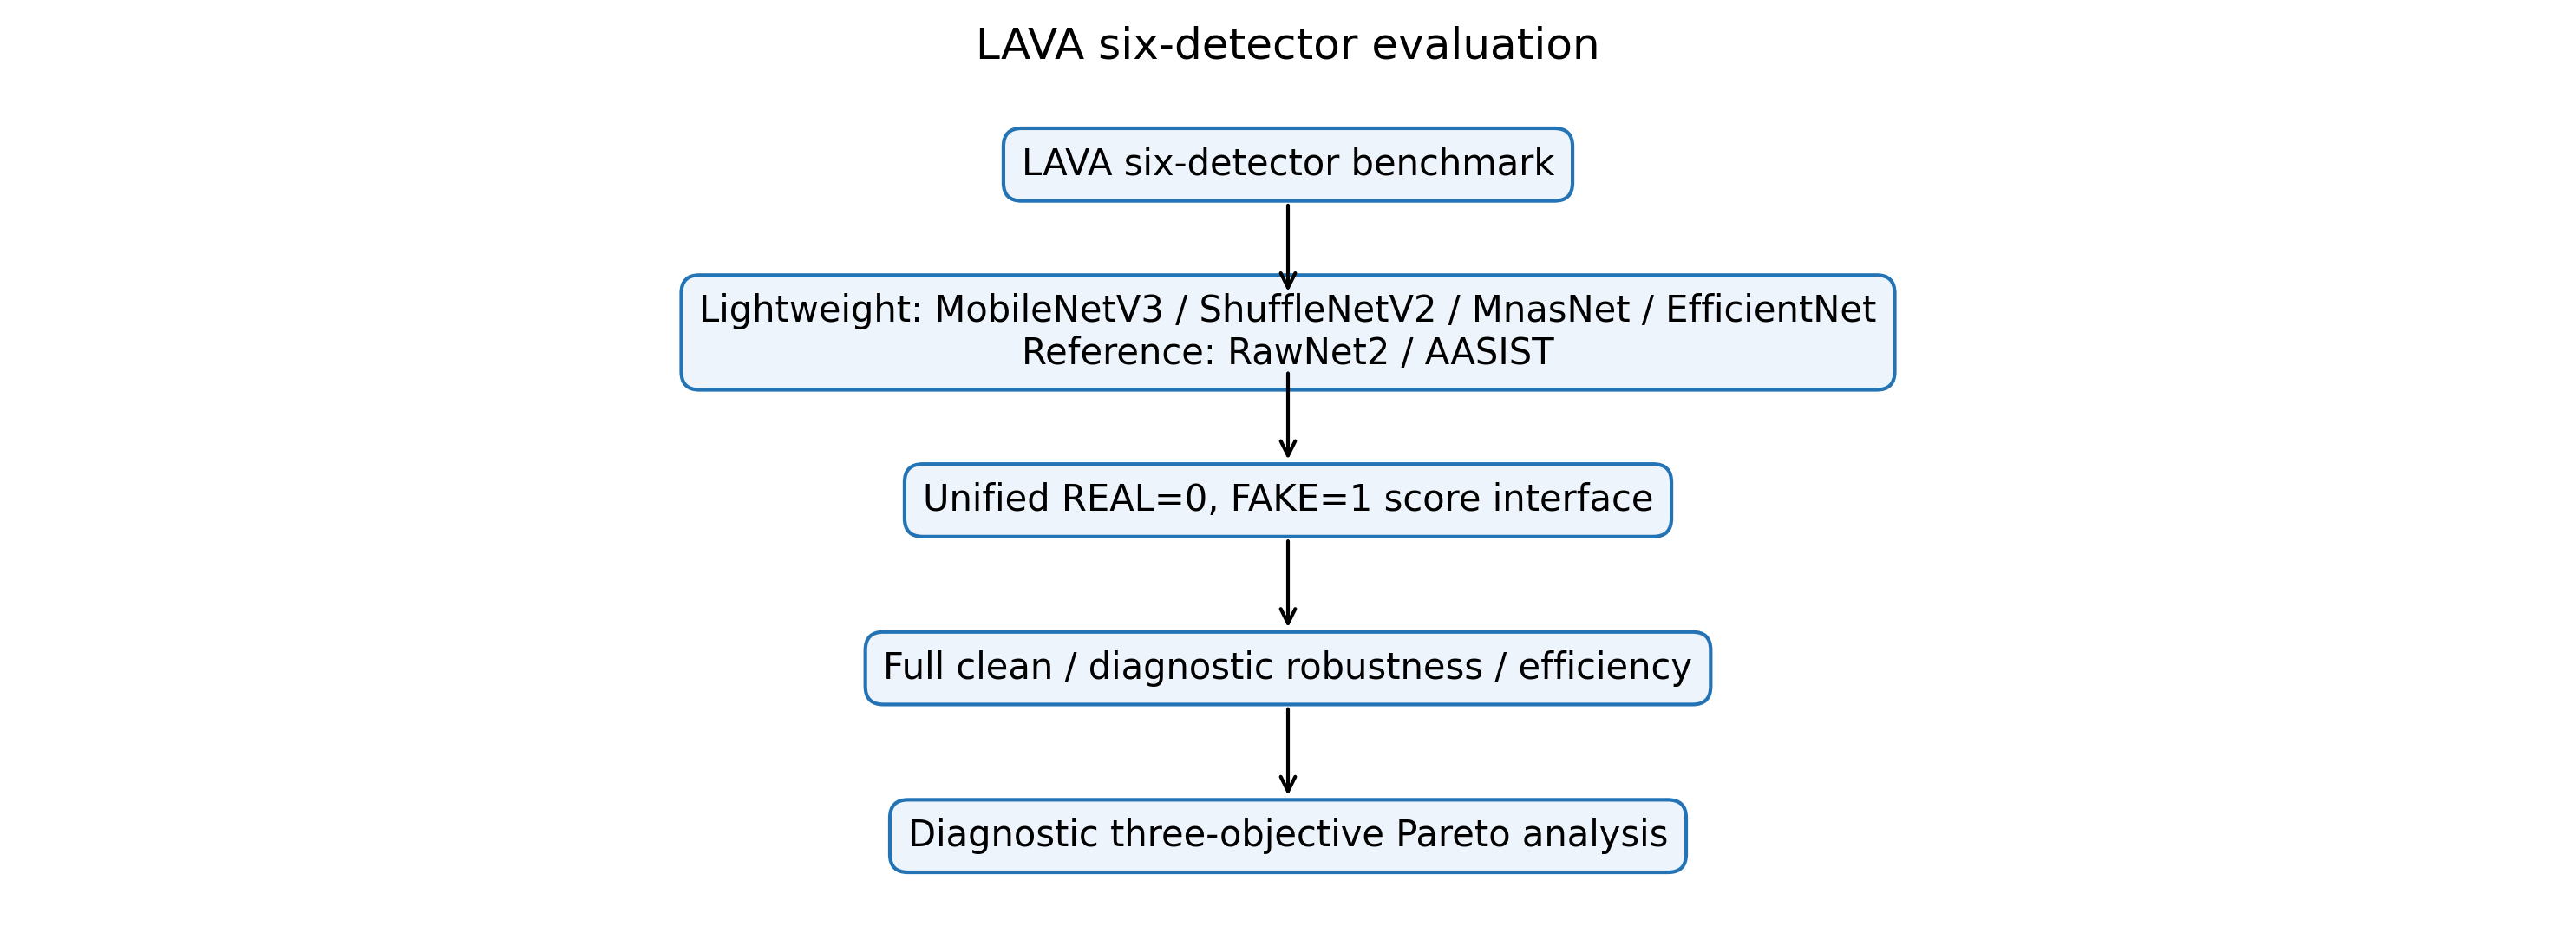
\includegraphics[width=.86\textwidth]{lava_6_model_overview.png}
\caption{Six native detectors connected to the unified LAVA evaluation boundary.}
\label{fig:overview}
\end{figure}

\subsection{Dataset Integrity and Canonical Split}
The internal binary collection has no speaker, source, generator, parent-recording, or dataset identifiers; LAVA therefore claims neither speaker-, source-, generator-, nor cross-dataset independence. It scanned 18,722 files (10,550 REAL, 8,172 FAKE), found 435 duplicate groups and 476 redundant files, and quarantined all 30 files in 14 cross-label checksum groups. Within a same-label group, the lexicographically first path is canonical. The retained 18,232 recordings comprise 10,493 REAL and 7,739 FAKE, split with seed 42 into 12,762/2,733/2,737 train/validation/test samples. The supported claim is \emph{checksum-group-disjoint only}. For $h(x)=\mathrm{SHA256}(x)$ and split group sets $G_s$,
\begin{equation}
x_i\sim x_j\!\iff\!h(x_i)=h(x_j),\qquad G_{tr}\cap G_{va}=G_{tr}\cap G_{te}=G_{va}\cap G_{te}=\varnothing .
\label{eq:integrity}
\end{equation}
The manifest hash is \nolinkurl{8b55591d58d3658b8cafe0e77b6ebdedbaa67be2e339730a7276fe9b10958df9}. Figure~\ref{fig:integrity} and Table~\ref{tab:data} record the implemented policy once.

Cross-label identity is handled more conservatively than ordinary duplication: every member of a conflicting checksum group is excluded, because a lexicographic representative would arbitrarily preserve one incompatible label. Same-label groups retain one representative to avoid weighting identical bytes multiple times. Split allocation operates on checksum groups, not paths, and the manifest checker recomputes both label conflicts and pairwise split intersections. This protocol prevents byte-level leakage but cannot detect perceptually duplicate re-encodings or shared speakers without additional metadata.

\begin{figure}[!t]
\centering
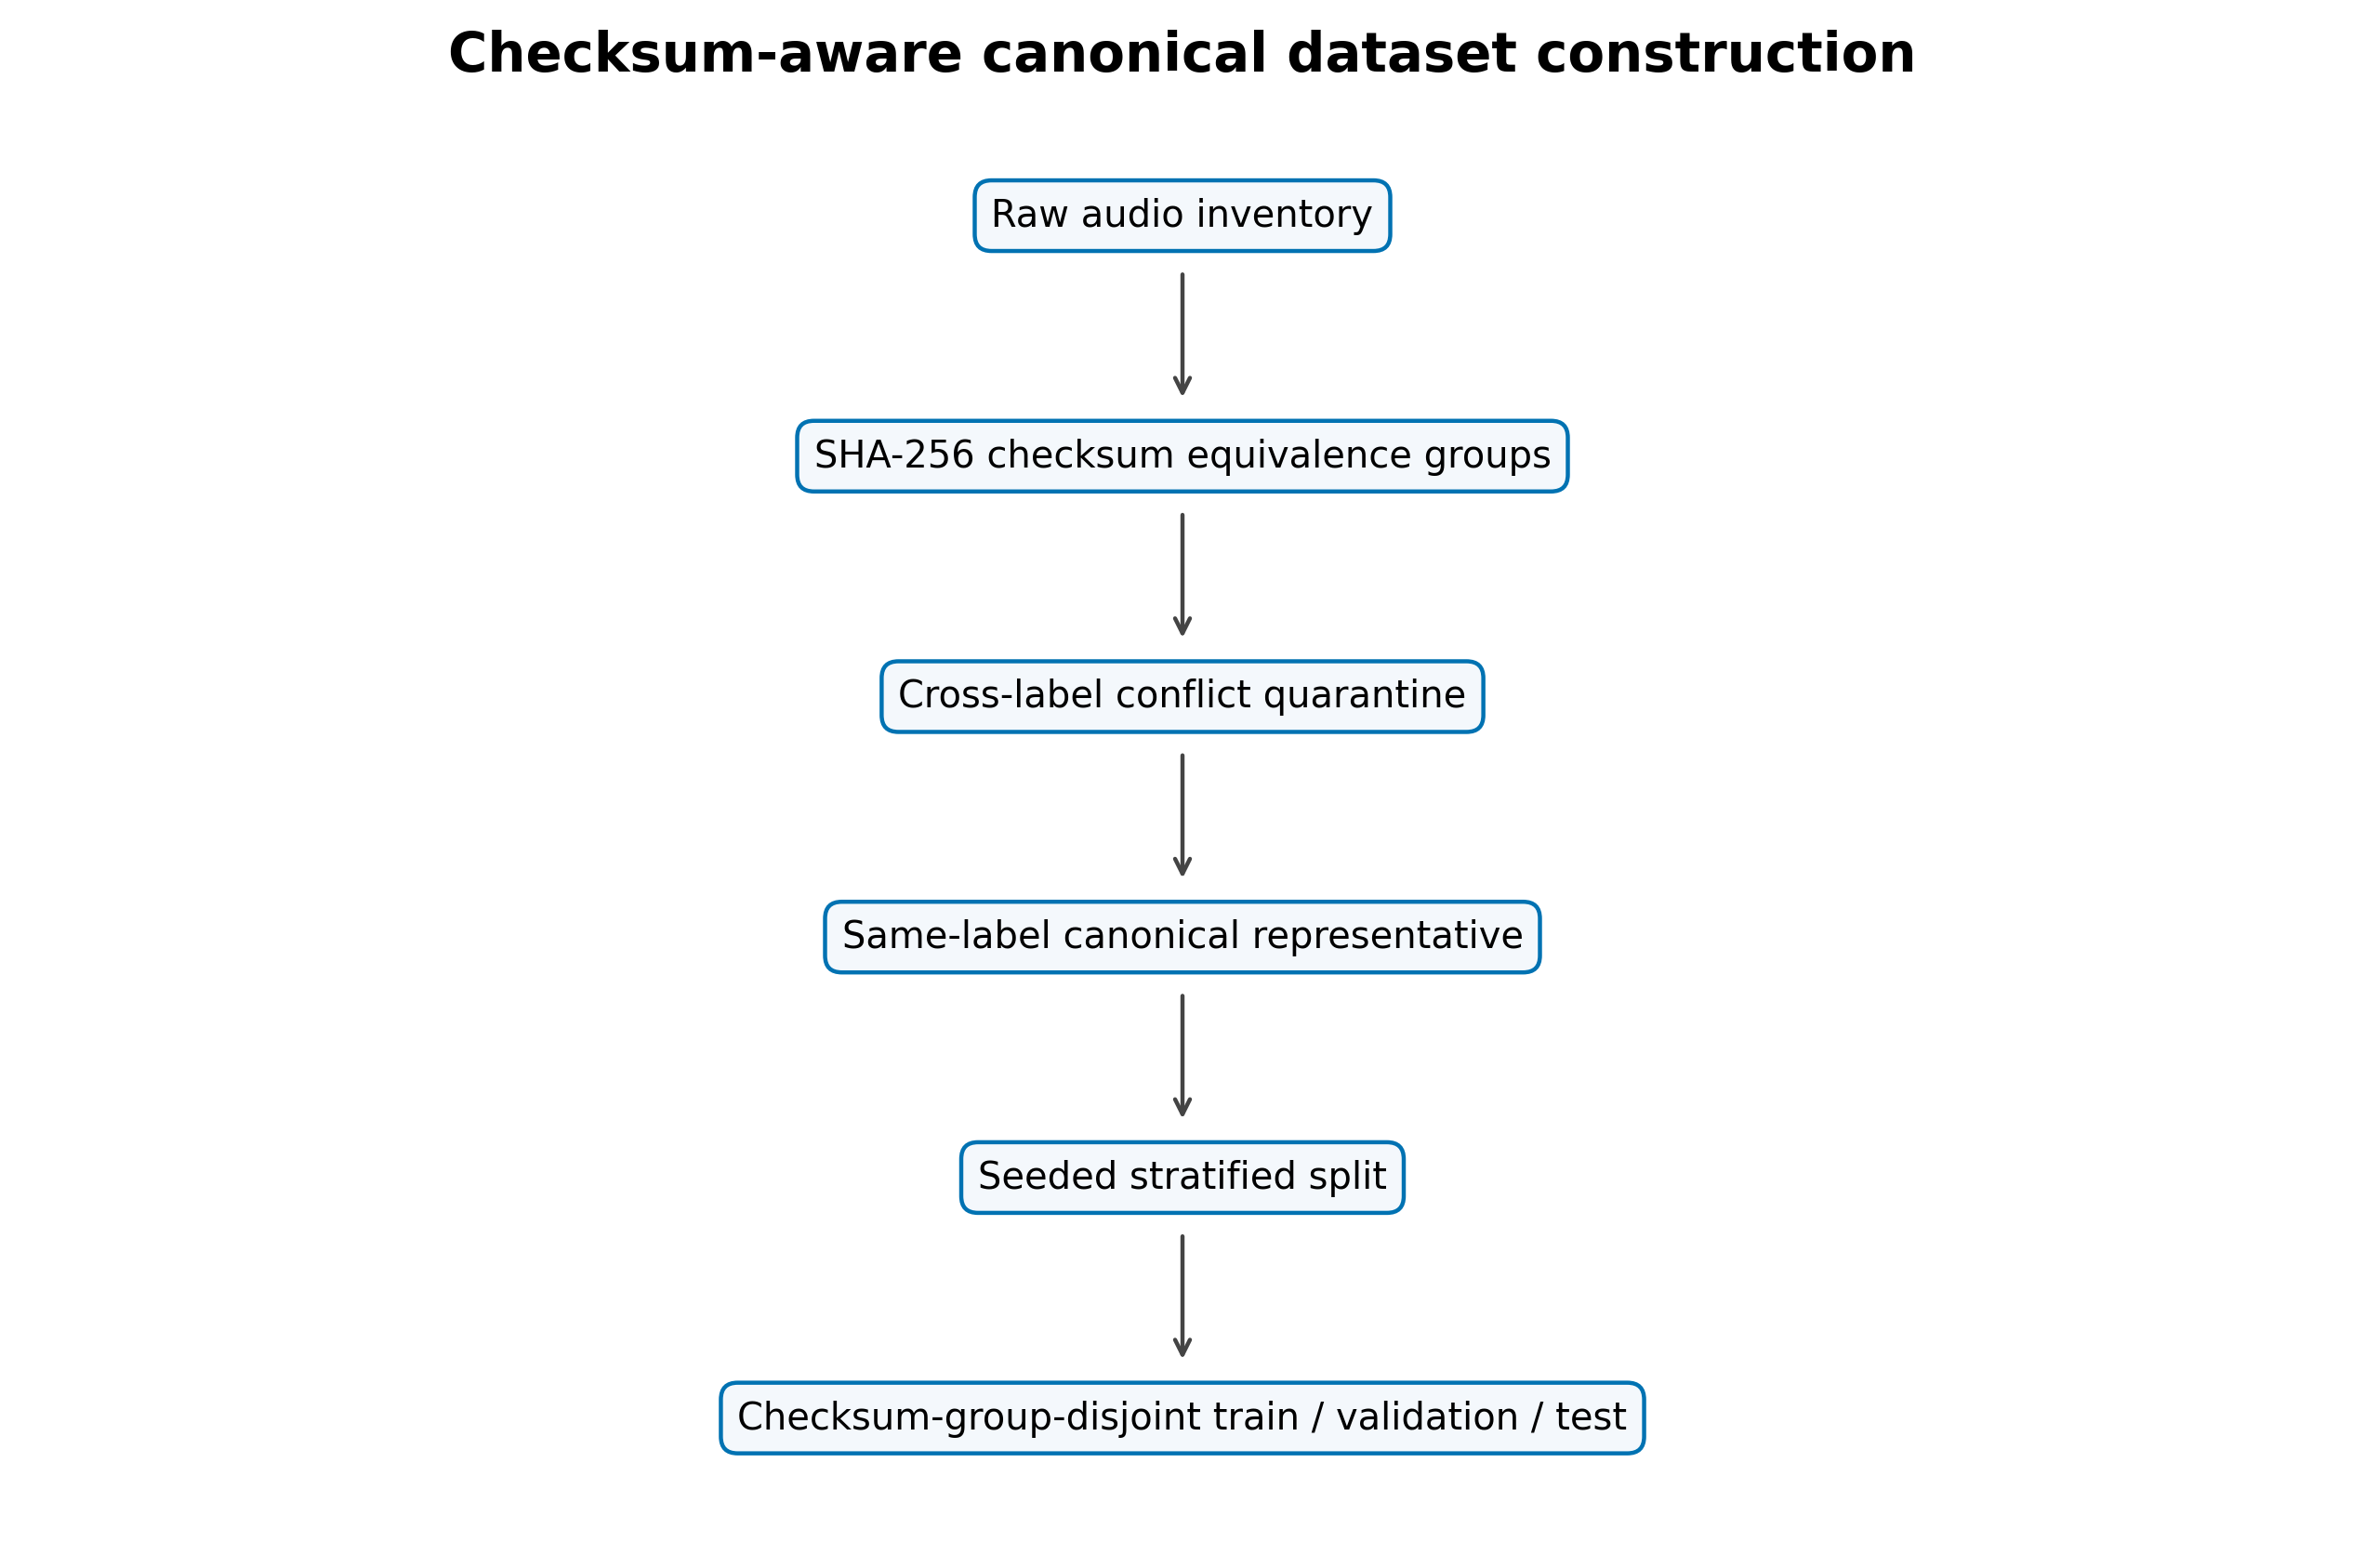
\includegraphics[width=.82\textwidth]{dataset_integrity_pipeline.png}
\caption{SHA-256 conflict quarantine, canonicalization, and disjoint splitting.}
\label{fig:integrity}
\end{figure}

\begin{table}[!t]
\centering\footnotesize
\caption{Canonical manifest and split inventory.}
\label{tab:data}
\begin{tabularx}{\textwidth}{Y r Y r}
\toprule
Inventory & Count & Split & Count \\
\midrule
Scanned / retained & 18,722 / 18,232 & Train & 12,762 \\
Retained REAL / FAKE & 10,493 / 7,739 & Validation & 2,733 \\
Duplicate groups / redundant & 435 / 476 & Test & 2,737 \\
Cross-label groups / files & 14 / 30 & Independence & checksum groups \\
\bottomrule
\end{tabularx}
\end{table}

\subsection{Standardized Audio Preprocessing}
Lightweight inputs are decoded, channel-averaged, polyphase-resampled to 22,050 Hz, and padded/truncated to 3.0 s. Six chronological 0.5-s segments use a Hann STFT ($N=2048$, hop 512), 128 HTK-style Mel filters spanning 20--8,000 Hz, relative dB mapping clipped to 80 dB, $[0,255]$ scaling, bilinear $224\times224$ resizing, and RGB replication. For segment $t$,
\begin{equation}
X_t(m,k)=\sum_{n=0}^{N-1}x_t[n+mH]w[n]e^{-j2\pi kn/N},\quad S_{t}^{mel}(m,r)=\sum_k|X_t(m,k)|^2H_r(k).
\label{eq:mel}
\end{equation}
The explicit SciPy/Mel implementation uses librosa only as a decoding fallback \cite{mcfee2015librosa}. Reference adapters instead consume mono 16-kHz waveforms of 64,600 samples (4.0375 s) using prefix/zero-padding. This documented difference is preserved rather than disguised as identical preprocessing.

Deterministic normalization precedes the six-way segmentation, so temporal order is never randomized. Segment dB values are referenced to that segment's maximum and floored before logarithmic conversion; the resulting image tensor has shape $6\times224\times224\times3$ in float32. Validation and test paths apply no stochastic augmentation. Reference repository padding may differ from LAVA's prefix/zero-padding for short clips; native-checkpoint/ONNX parity therefore verifies export fidelity on identical adapter tensors, not equivalence to the original authors' full preprocessing pipeline.

\subsection{Evaluated Detector Architectures}
For the lightweight family, shared segment encoder $f_\theta$ produces six embeddings, an LSTM with 128 units aggregates them, and a 64-unit ReLU layer plus dropout 0.4 feeds a sigmoid:
\begin{equation}
p_{fake}=\sigma\!\left(W_2\,\mathrm{Dropout}_{.4}\!\left(\mathrm{ReLU}(W_1\mathrm{LSTM}(f_\theta(X_{1:6}))+b_1)\right)+b_2\right).
\label{eq:head}
\end{equation}
MobileNetV3 uses inverted residual and squeeze--excitation blocks; ShuffleNetV2 uses channel split/shuffle; MnasNet provides platform-searched inverted residual stages; EfficientNet-B0 uses compound scaling and MBConv blocks. RawNet2 retains its Sinc-style front end, residual blocks, attention, GRU, and classifier; AASIST retains spectral--temporal heterogeneous graph attention and readout. Figure~\ref{fig:archprov} combines the common lightweight path with the unequal provenance that must qualify comparisons.

Backbone embeddings are not artificially equalized: MobileNetV3 exposes 576 dimensions, ShuffleNetV2 1,024, and MnasNet/EfficientNet 1,280. TimeDistributed shares one backbone across all six segments, so parameters are not multiplied by six even though per-recording convolutional work is. RawNet2 instead learns directly from waveform samples through a Sinc-style filter bank and residual temporal hierarchy before GRU classification. AASIST constructs spectral and temporal graphs, performs graph attention and heterogeneous interaction with master nodes, and pools them for classification. LAVA changes neither reference topology into a Mel-CNN-LSTM.

MobileNetV3Small couples inverted residual bottlenecks with squeeze--excitation and hardware-aware nonlinearities and yields the narrowest segment embedding. ShuffleNetV2's stride-one units preserve one channel branch while transforming the other with pointwise/depthwise/pointwise convolutions; concatenation and channel shuffle exchange features, whereas stride-two units transform both branches. MnasNet-A1 and EfficientNet-B0 both use mobile inverted bottlenecks but originate from different search/scaling criteria. These implementation details matter because four backbones with a common recurrent head do not constitute the same capacity or optimization landscape.

The reference family establishes a deliberately different comparison stratum. RawNet2's learned band-limited front end, residual temporal blocks, channel attention, and GRU operate over 64,600 samples. AASIST forms two-dimensional features, spectral and temporal graphs, heterogeneous graph interactions, master nodes, and graph pooling before its classifier. Their source repositories associate the checkpoints with ASVspoof 2019 LA, but neither was trained from scratch using the canonical LAVA train split. They are therefore described as externally pretrained reference anti-spoofing artifacts throughout.

\begin{figure}[!t]
\centering
\begin{minipage}{.49\textwidth}\centering
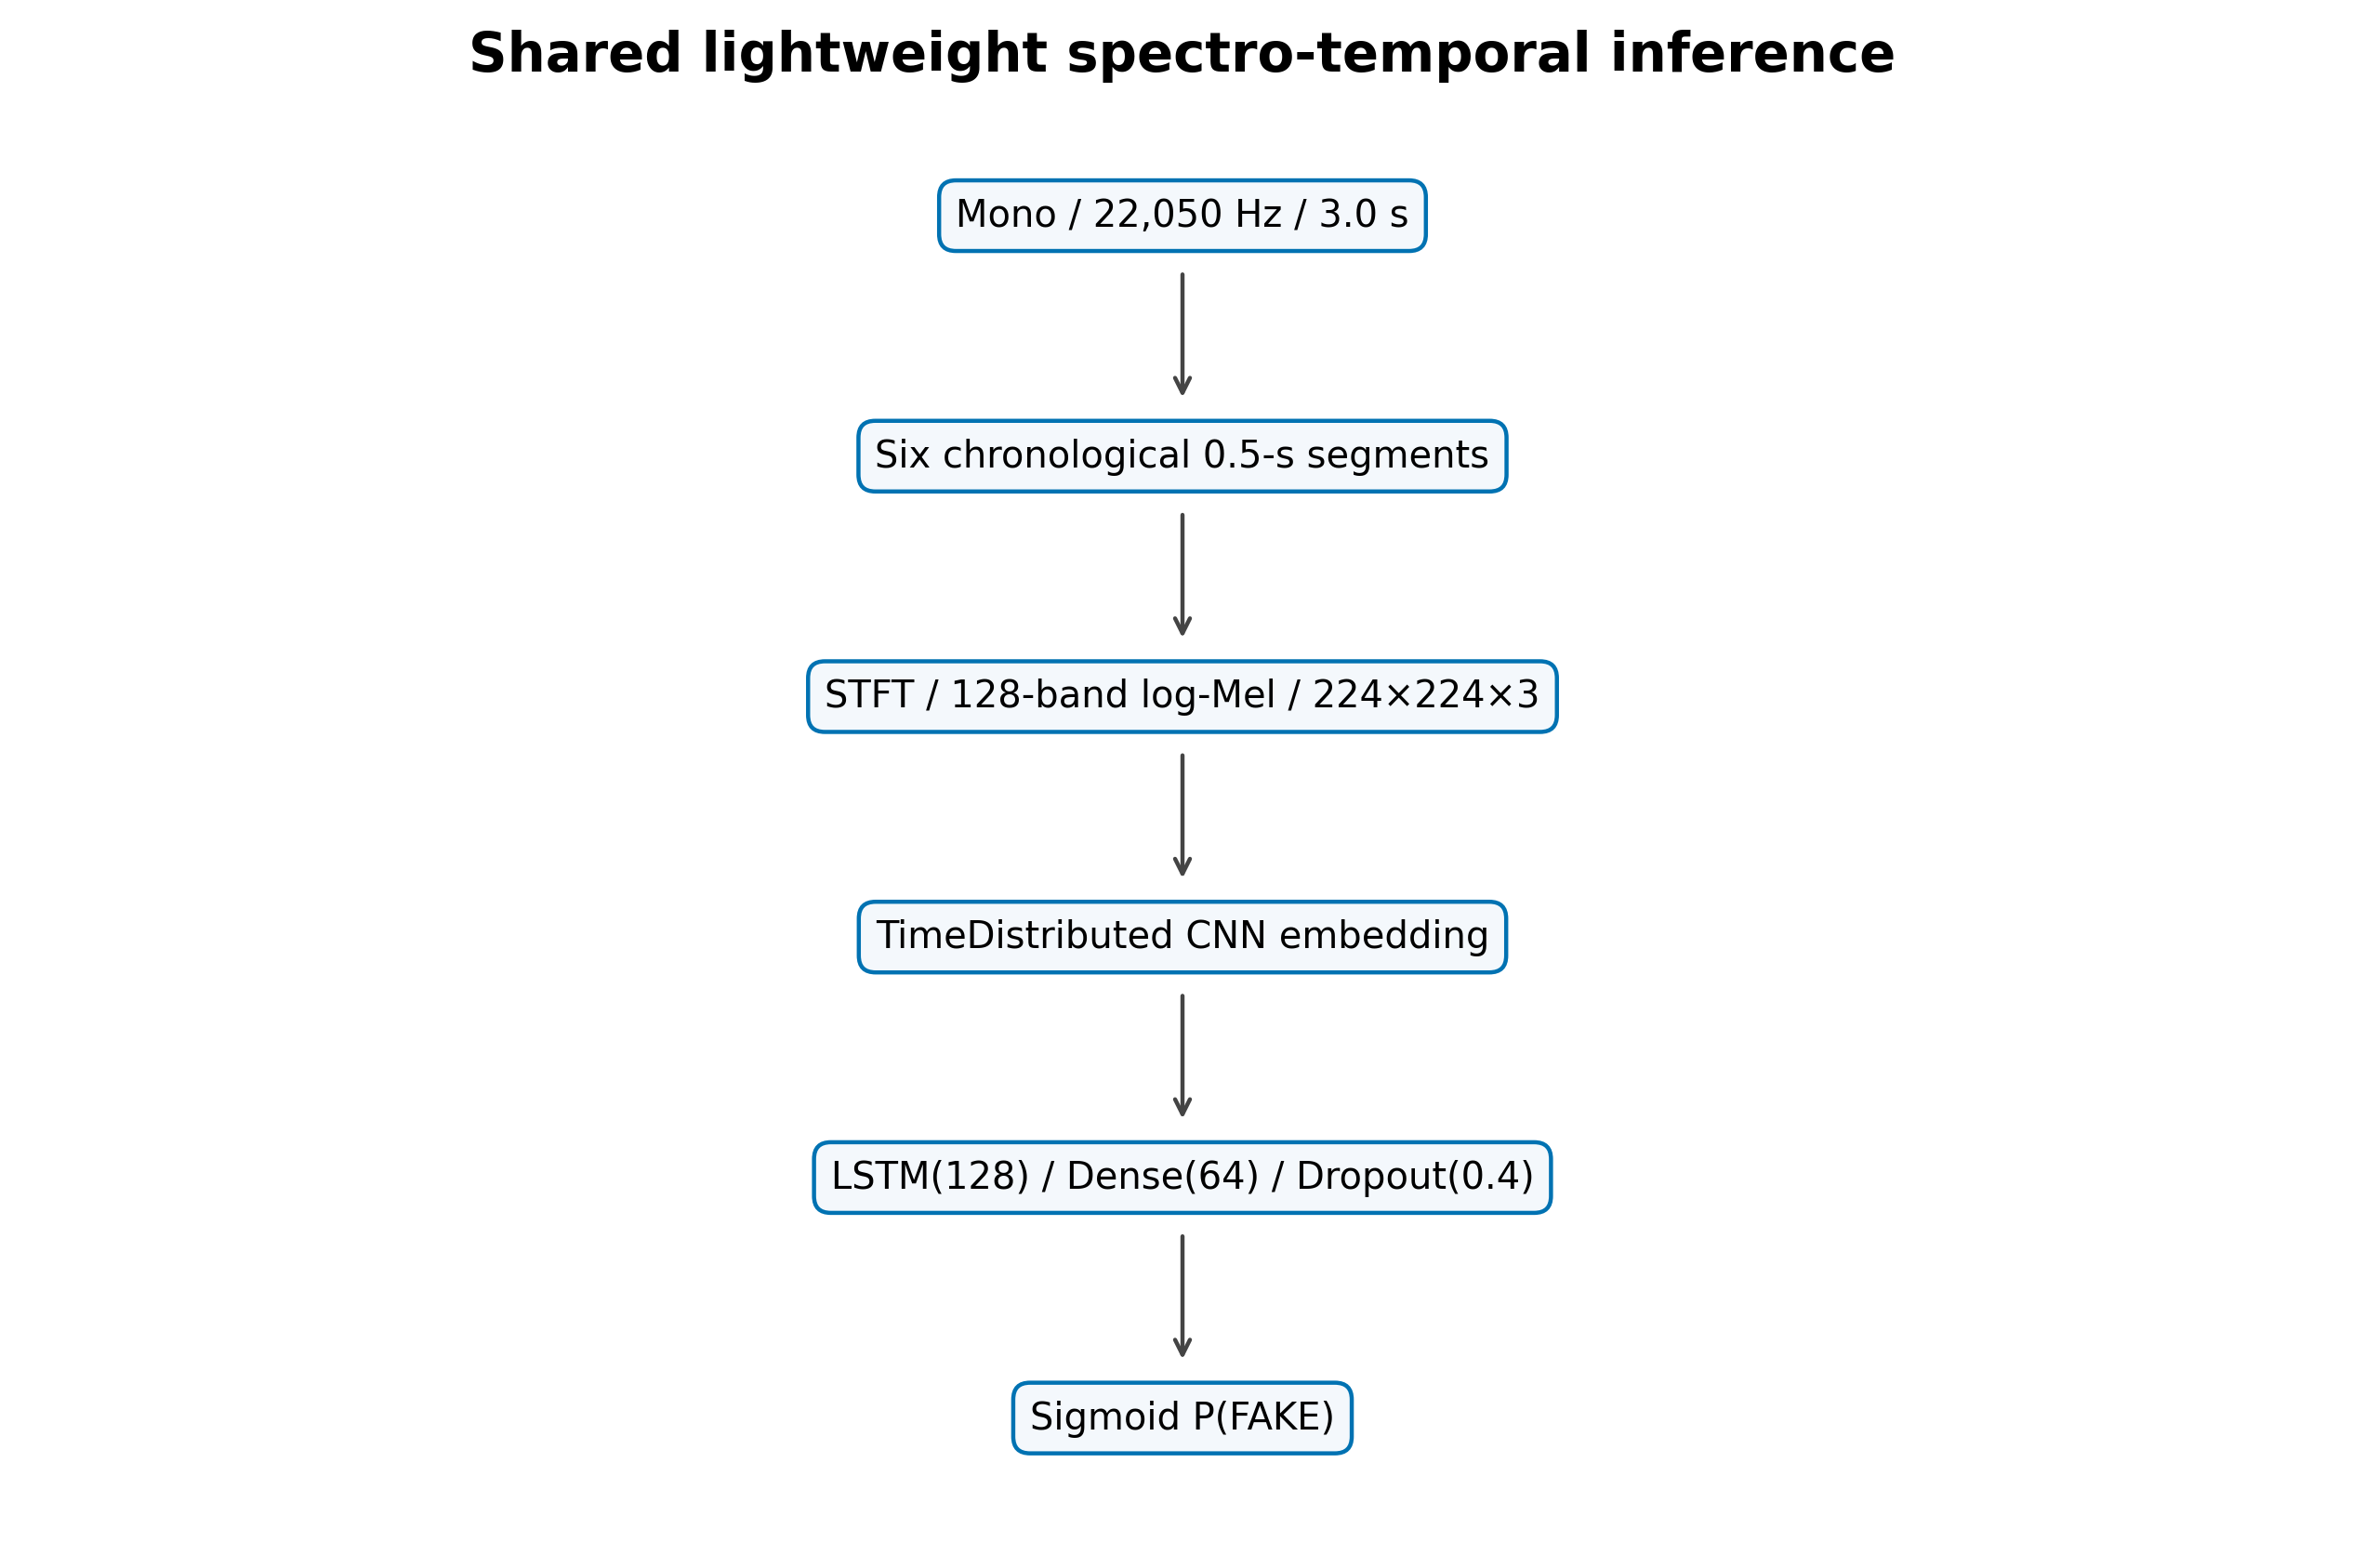
\includegraphics[width=\linewidth]{lightweight_temporal_pipeline.png}\\[-1mm]\small (a) Mel-sequence temporal path
\end{minipage}\hfill
\begin{minipage}{.49\textwidth}\centering
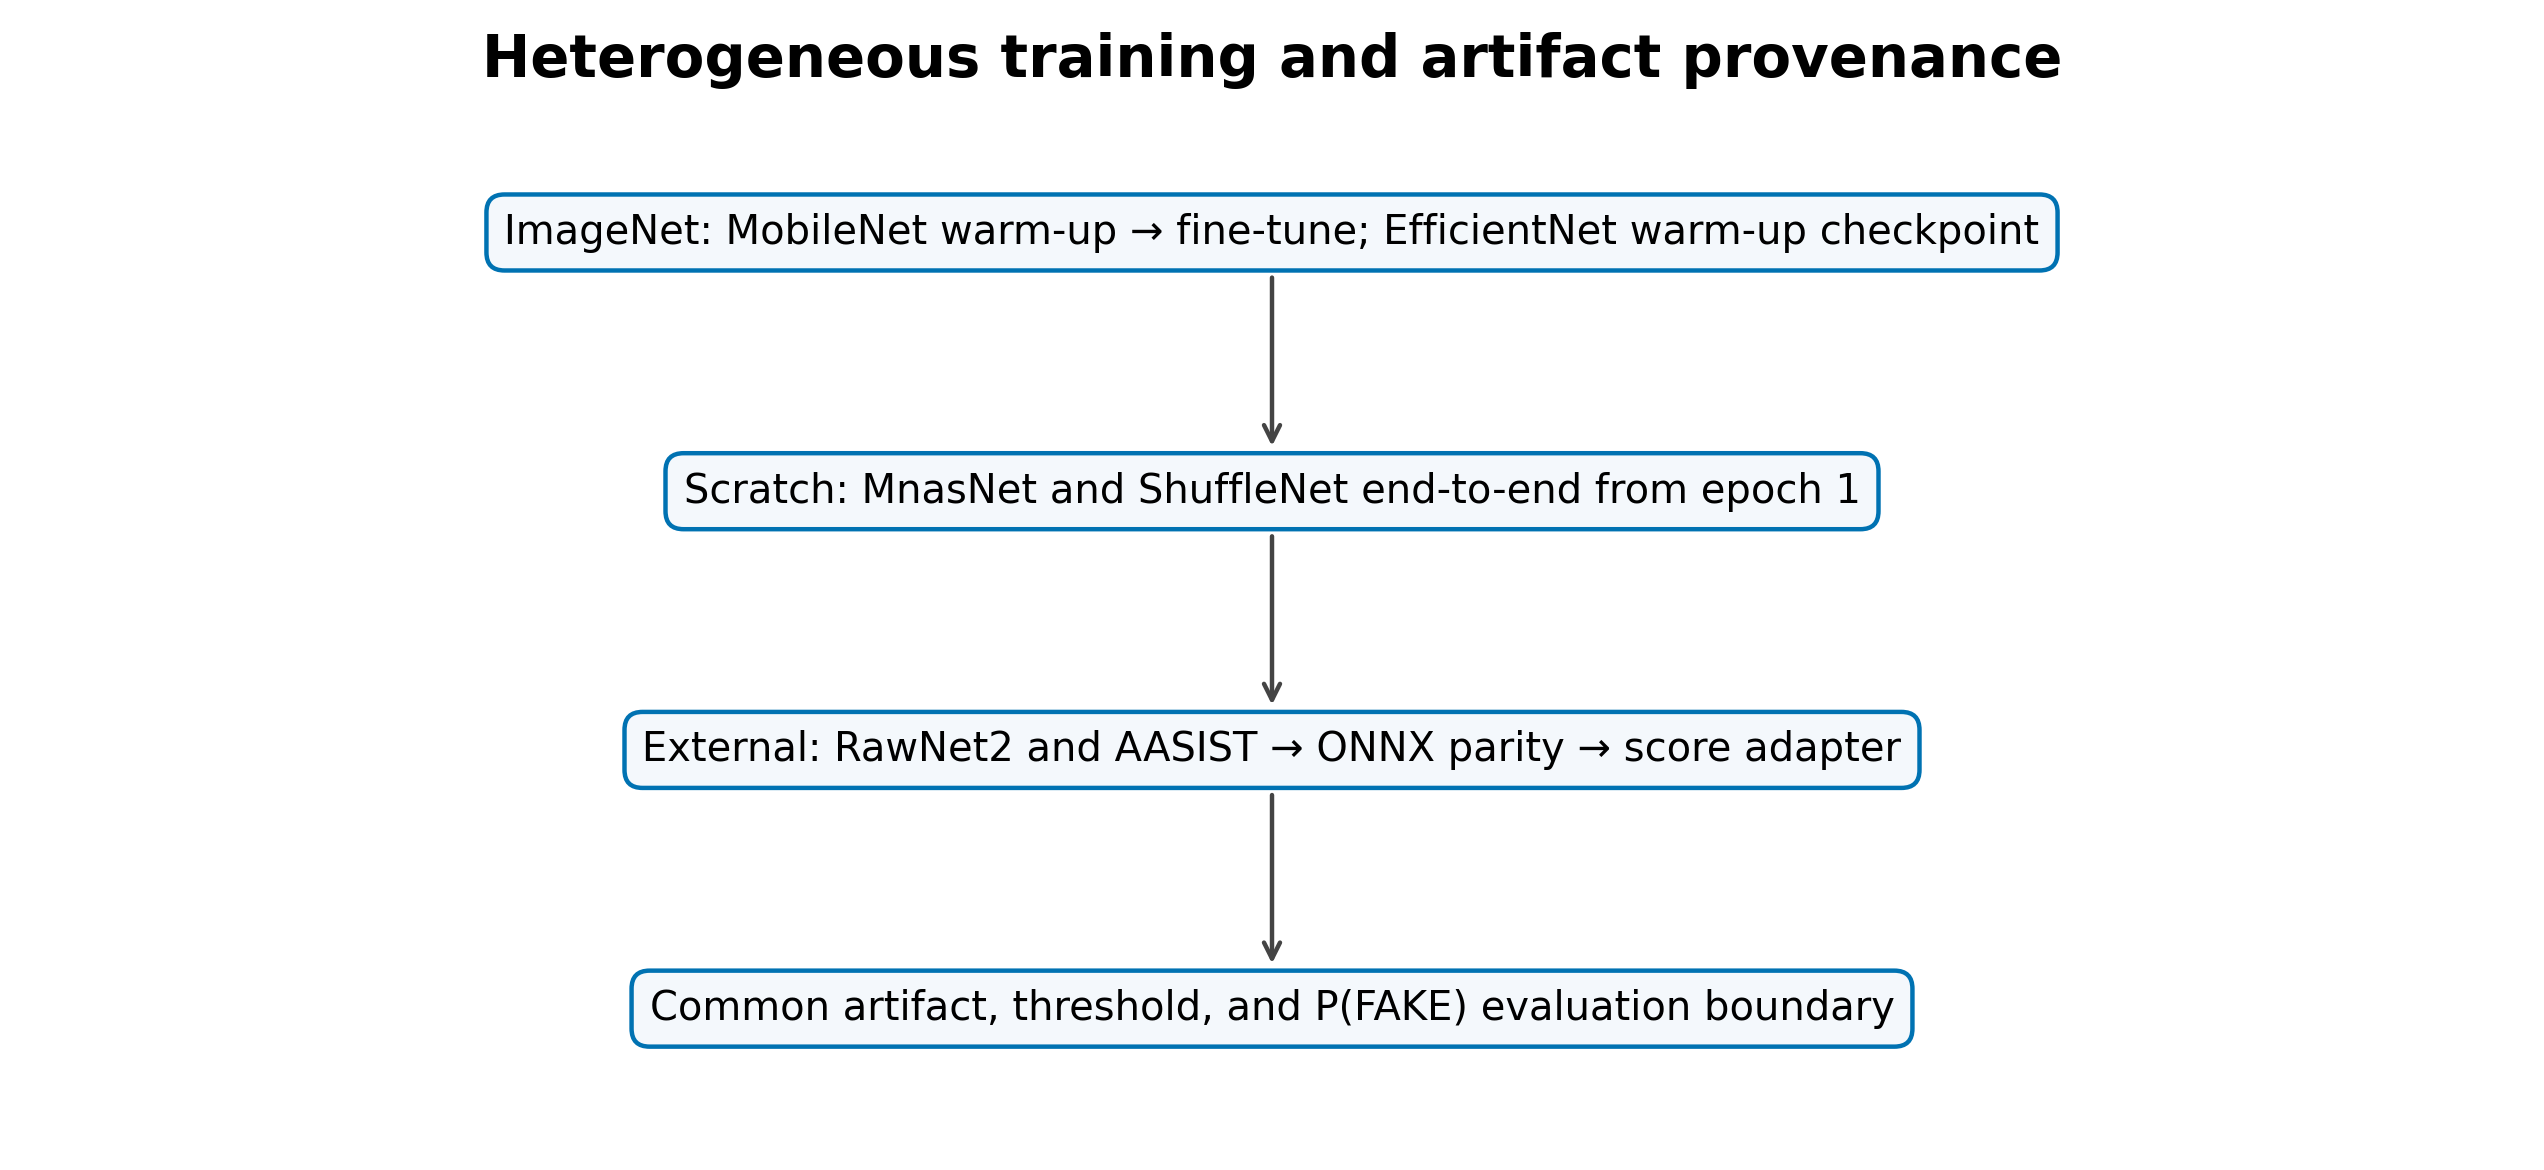
\includegraphics[width=\linewidth]{training_provenance_strategies.png}\\[-1mm]\small (b) Artifact provenance
\end{minipage}
\caption{Architecture and provenance: the evaluation contract is shared, training is not.}
\label{fig:archprov}
\end{figure}

\begin{table}[!t]
\centering\scriptsize
\caption{Detector specification, provenance, and deployed threshold.}
\label{tab:models}
\begin{tabularx}{\textwidth}{l l l r Y l}
\toprule
Detector & Input & Temporal core & Params & Initialization/artifact provenance & $\tau$ \\
\midrule
MobileNetV3-LSTM & Mel, 3.0 s & LSTM(128) & 1,308,401 & ImageNet; warm-up + partial fine-tune & .82 \\
ShuffleNetV2-LSTM & Mel, 3.0 s & LSTM(128) & 1,868,441 & scratch; full end-to-end, best epoch 16/28 & .12 \\
MnasNet-A1-LSTM & Mel, 3.0 s & LSTM(128) & 3,369,255 & scratch; full end-to-end, best epoch 27/39 & .90 \\
EfficientNet-B0-LSTM & Mel, 3.0 s & LSTM(128) & 4,779,300 & ImageNet; best warm-up epoch 47 & .90 \\
RawNet2 & waveform, 4.04 s & GRU & 17,621,410 & external reference; ONNX export & .50 \\
AASIST & waveform, 4.04 s & graph readout & 297,866 & external reference; ONNX export & .50 \\
\bottomrule
\end{tabularx}
\end{table}

\subsection{Training, Artifact Provenance, and Score Semantics}
MobileNet and EfficientNet use ImageNet initialization; EfficientNet's deployment is explicitly the best warm-up checkpoint, not a completed fine-tuning lifecycle. MnasNet and ShuffleNet were trained jointly with their recurrent heads from scratch; all 49 and 56 BatchNormalization layers, respectively, were trainable from epoch 1. RawNet2 and AASIST were not trained by LAVA: strict PyTorch loading followed by ONNX export gave maximum native/export score differences of $4.11\times10^{-6}$ and $5.96\times10^{-8}$ on six real tensors. This verifies conversion, not identical training or publication-pipeline equivalence.

MobileNet followed frozen-backbone warm-up and lower-rate partial fine-tuning with BatchNormalization frozen. EfficientNet's selected warm-up checkpoint is epoch 47 (validation loss 0.1698). MnasNet used Adam from $10^{-4}$, stopped at epoch 39, and restored epoch 27. ShuffleNet used Adam from $3\times10^{-4}$, stopped at epoch 28, and restored epoch 16; its backbone and all BatchNormalization layers remained trainable. Thus the common evaluation boundary provides matched testing, not a controlled comparison of initialization or optimization.

LAVA fixes REAL=0 and FAKE=1; every adapter returns $p=P(\mathrm{FAKE})$ and
\begin{equation}
\hat y=\mathbf{1}[p\ge\tau],\qquad \tau^*=\arg\max_{\tau}F1_{val}(\tau).
\label{eq:decision}
\end{equation}
The four lightweight thresholds in Table~\ref{tab:models} use validation only. External references retain uncalibrated defaults of 0.5. Test labels select neither thresholds nor weights, and scores are not claimed to be calibrated real-world probabilities.

Threshold calibration maximizes validation FAKE-class F1 over the configured grid and is stored beside the artifact. Consequently, a score below a high threshold may be labeled REAL even when $p>0.5$; the UI reports the raw score and decision boundary rather than presenting $1-p$ as calibrated confidence. ROC-AUC is always calculated from raw $P(\mathrm{FAKE})$, and EER is likewise threshold-independent with respect to the deployed operating point. These conventions avoid silently reversing native class orders: the TensorFlow sigmoid already represents FAKE, while the reference adapters select the checkpoint-defined spoof index before exposing the common score.

\subsection{Clean and Robustness Evaluation}
Clean evaluation uses all 2,737 test samples (1,575 REAL, 1,162 FAKE). Accuracy, classwise and macro F1, ROC-AUC from raw scores, and linearly interpolated EER are reported. With FAKE positive,
\begin{equation}
P=\frac{TP}{TP+FP},\ R=\frac{TP}{TP+FN},\ F1=\frac{2PR}{P+R};\quad FAR=\frac{FP}{FP+TN},\ FRR=\frac{FN}{FN+TP},\ EER\simeq\frac{FAR+FRR}{2}.
\label{eq:metrics}
\end{equation}
The EER implementation sorts distinct raw-score thresholds, forms FAR and FRR, finds the first sign change of $FAR-FRR$, and linearly interpolates the crossing; if no sign change occurs, it uses the minimum absolute gap. Confusion counts use the stored deployed threshold and are therefore operating-point dependent, whereas ROC-AUC and EER characterize score ordering. Macro-F1 gives equal weight to REAL and FAKE and supplements the positive-class F1 used during lightweight threshold selection.
Robustness uses a preselected stratified subset of 100 test recordings (58 REAL, 42 FAKE; seed 42), and each baseline uses those same IDs. Four seeded AWGN levels (20, 10, 5, 0 dB) use sample-identity-derived seeds. FFmpeg round trips cover MP3 128/64 kb/s, Opus 64 kb/s, and AAC 96 kb/s. Simulated replay applies taps at 0/17/43/89 ms with gains 1/.45/.25/.12, normalization by 1.82, and a causal fourth-order 100--3,800-Hz band-pass. It is not physical replay. For nine conditions,
\begin{equation}
\Delta F1_k=F1_{clean}-F1_k,\qquad \overline{\Delta F1}=\frac{1}{9}\sum_{k=1}^{9}\Delta F1_k.
\label{eq:degradation}
\end{equation}
Negative degradation means improvement on this small subset and is not automatically robustness. Full-test stress, physical replay, and unseen evaluation are respectively \texttt{NOT\_RUN}, \texttt{NOT\_AVAILABLE}, and \texttt{NOT\_AVAILABLE}.

Noise power is derived from each clean signal's measured power, and the first 16 hexadecimal characters of its SHA-256 identity determine its random seed. Stress waveforms are materialized once and shared by every adapter. Codec audio is converted to PCM16, encoded, decoded, and re-entered through the ordinary model path; the codec-library version was not sealed and is therefore \texttt{NOT\_MEASURED}. These controls isolate detector differences from independently sampled or re-encoded perturbations.

\subsection{Efficiency, Statistics, and Pareto Analysis}
Each artifact runs float32, batch one, one backend thread, and no accelerator in a sequential isolated process on the same Windows AMD64 desktop CPU. Ten warm-ups precede 50 timed repetitions. Measurements separate preprocessing, model-only, and end-to-end time and include P95, load time, throughput, and whole-process RSS. The commercial CPU name and installed RAM were not recorded. For $N$ clips,
\begin{equation}
Q=\frac{N}{T_{total}},\qquad RTF=\frac{T_{processing}}{T_{audio}}.
\label{eq:efficiency}
\end{equation}
RTF below one demonstrates faster-than-duration offline processing, not causal streaming or edge deployment.

The runner reports preprocessing and model-only time in addition to end-to-end mean, P95, throughput, load time, and RSS sampled every 20 ms. Interpreter start-up and graph tracing are excluded from warm timing. Keras parameter counts include non-trainable BatchNormalization state, whereas native PyTorch reference counts exclude buffers; serialized size and executed latency therefore remain separate reported quantities.

Model-only and end-to-end repetitions are warmed independently. Timing synchronizes execution by materializing returned arrays before stopping the clock, avoiding asynchronous dispatch being mistaken for completion. Throughput is the reciprocal of aggregate end-to-end duration rather than the reciprocal of a rounded mean. The RTF denominator follows each detector's declared duration (3.0 s for lightweight models and 4.0375 s for references). Hence RTF supports within-protocol deployment comparison but does not erase input-duration differences.

The six full-test score files are joined by sample ID. One thousand class-stratified bootstrap replicates (seed 42) give percentile 95\% intervals for F1, AUC, and EER \cite{efron1979bootstrap}. Exact McNemar tests compare paired correctness \cite{mcnemar1947}; Holm correction covers all 15 pairs \cite{holm1979}. Agreement is the proportion of identical decisions. These are test-sample, not multi-seed, uncertainties. Diagnostic Pareto objectives minimize subset EER, mean $\Delta F1$, and end-to-end RTF. Model $A$ dominates $B$ iff
\begin{equation}
f_i(A)\le f_i(B)\ \forall i\quad\mathrm{and}\quad\exists j:f_j(A)<f_j(B).
\label{eq:pareto}
\end{equation}
No weighted score is used. Because robustness covers 100 recordings, this frontier is exploratory; an official full-test frontier remains \texttt{NOT\_RUN}. Per-sample scores, hashes, complete statistics, and generation scripts remain in the repository supplement.

Bootstrap resampling preserves the observed class counts by drawing REAL and FAKE indices independently and then recombining them, so a replicate cannot accidentally lose a class. Pairwise F1-difference intervals reuse the same resampled IDs for both models, preserving dependence. McNemar counts only discordant correctness outcomes and asks whether their directions are symmetric; Holm's sequential adjustment controls family-wise error without assuming detector independence. Agreement and error-overlap analyses are descriptive complements, not significance tests.

Reproducibility is organized around immutable evidence rather than manuscript numbers. Canonical clean outputs contain 2,737 score rows per detector under \texttt{outputs/lava\_6/clean}; robustness outputs preserve the 100 selected sample IDs and condition manifest; efficiency summaries seal warm-up/run counts and thread policy. Aggregate tables are generated from these CSV/JSON files without importing detector loaders, so paper generation cannot trigger model execution. The detector registry and production UI use packaged metadata when ignored benchmark outputs are absent on deployment. Acceptance checks require six clean and efficiency rows, six entries for every completed stress condition, a $6\times6$ agreement matrix, and six Pareto inputs. Historical five-model outputs remain unchanged, allowing the incremental addition of ShuffleNet to be audited.

The clean and diagnostic scopes are intentionally separated in filenames, summaries, and language. Full-test EER appears in clean performance and bootstrap reporting; subset EER is used only in the diagnostic Pareto vector because the corresponding robustness coordinate uses the same 100 IDs. Mixing full-test EER with subset degradation would produce a numerically valid but scope-inconsistent frontier. Likewise, the 100-sample clean baseline is never substituted for the 2,737-sample clean table. This scope discipline is part of the benchmark contract, not merely a reporting convention.

\section{Results and Discussion}
\subsection{Clean Detection Performance (RQ1)}
All six artifacts passed load, finite bounded-score, hash, and adapter checks. Table~\ref{tab:clean} reports the full canonical test. ShuffleNet led every aggregate (F1 0.9824, macro-F1 0.9847, AUC 0.9929, EER 0.0146) with 24 false positives and 17 false negatives. MobileNet ranked second on F1 and AUC, followed by MnasNet and the available EfficientNet warm-up checkpoint. RawNet2 and AASIST were near chance under this dataset/adapter contract. This is not an architecture-only ranking because provenance, duration, representation, threshold calibration, and training differ.

Class-wise counts refine the aggregate view. MobileNet produced 30 false positives and 34 false negatives. MnasNet traded more false positives (47) for fewer false negatives (36), whereas EfficientNet's 31/69 split shows that its principal error was missed FAKE speech at the validation-selected threshold. RawNet2 generated 1,015 false positives and 371 false negatives; AASIST generated 715 and 513. These reference outcomes are consistent with score/domain mismatch and uncalibrated default thresholds, but the present evidence cannot attribute them to one cause.

The associated REAL/FAKE F1 values were 0.9797/0.9724 for MobileNet, 0.9870/0.9824 for ShuffleNet, 0.9736/0.9645 for MnasNet, and 0.9686/0.9563 for EfficientNet. The reference values were 0.4469/0.5330 for RawNet2 and 0.5834/0.5139 for AASIST. Reporting both classes prevents the positive-class F1 from hiding RawNet2's asymmetric tendency to label REAL recordings as FAKE. Confusion counts and class-wise values remain reproducible from the full score CSV rather than a normalized image.

\begin{table}[!t]
\centering\scriptsize
\caption{Clean performance on all 2,737 canonical test recordings.}
\label{tab:clean}
\begin{tabularx}{\textwidth}{l r r r r r r r}
\toprule
Model & Acc. & Prec. & Rec. & F1 & Macro-F1 & AUC & EER \\
\midrule
MobileNetV3 & .9766 & .9741 & .9707 & .9724 & .9761 & .9911 & .0250 \\
ShuffleNetV2 & .9850 & .9795 & .9854 & .9824 & .9847 & .9929 & .0146 \\
MnasNet-A1 & .9697 & .9599 & .9690 & .9645 & .9690 & .9886 & .0310 \\
EfficientNet-B0 & .9635 & .9724 & .9406 & .9563 & .9624 & .9877 & .0400 \\
RawNet2 ext. & .4936 & .4380 & .6807 & .5330 & .4900 & .5178 & .4813 \\
AASIST ext. & .5513 & .4758 & .5585 & .5139 & .5487 & .5597 & .4463 \\
\bottomrule
\end{tabularx}
\end{table}
Raw-score ROC and DET views in Fig.~\ref{fig:clean} separate threshold-independent discrimination from deployed decisions. The four lightweight curves are strong; the reference curves are close to diagonal. Bootstrap intervals overlap among some lightweight systems, so close AUC values are not presented as universal ranks.

Artifact checks also constrain interpretation of this gap. ShuffleNet's TensorFlow 2.15 conversion reproduced source scores within $1.75\times10^{-10}$ and matched the canonical training-manifest hash. The reference ONNX exports matched their native checkpoints within the tolerances reported in Section III-E, making gross serialization or class-index reversal unlikely. Nevertheless, validation-calibrated lightweight thresholds and uncalibrated reference thresholds affect confusion metrics, while domain and preprocessing shifts affect both thresholded and raw-score measures. The results therefore support a statement about the deployed artifacts under LAVA, not about the maximum attainable RawNet2 or AASIST performance after retraining or calibration.

\begin{figure}[!t]
\centering
\begin{minipage}{.49\textwidth}\centering
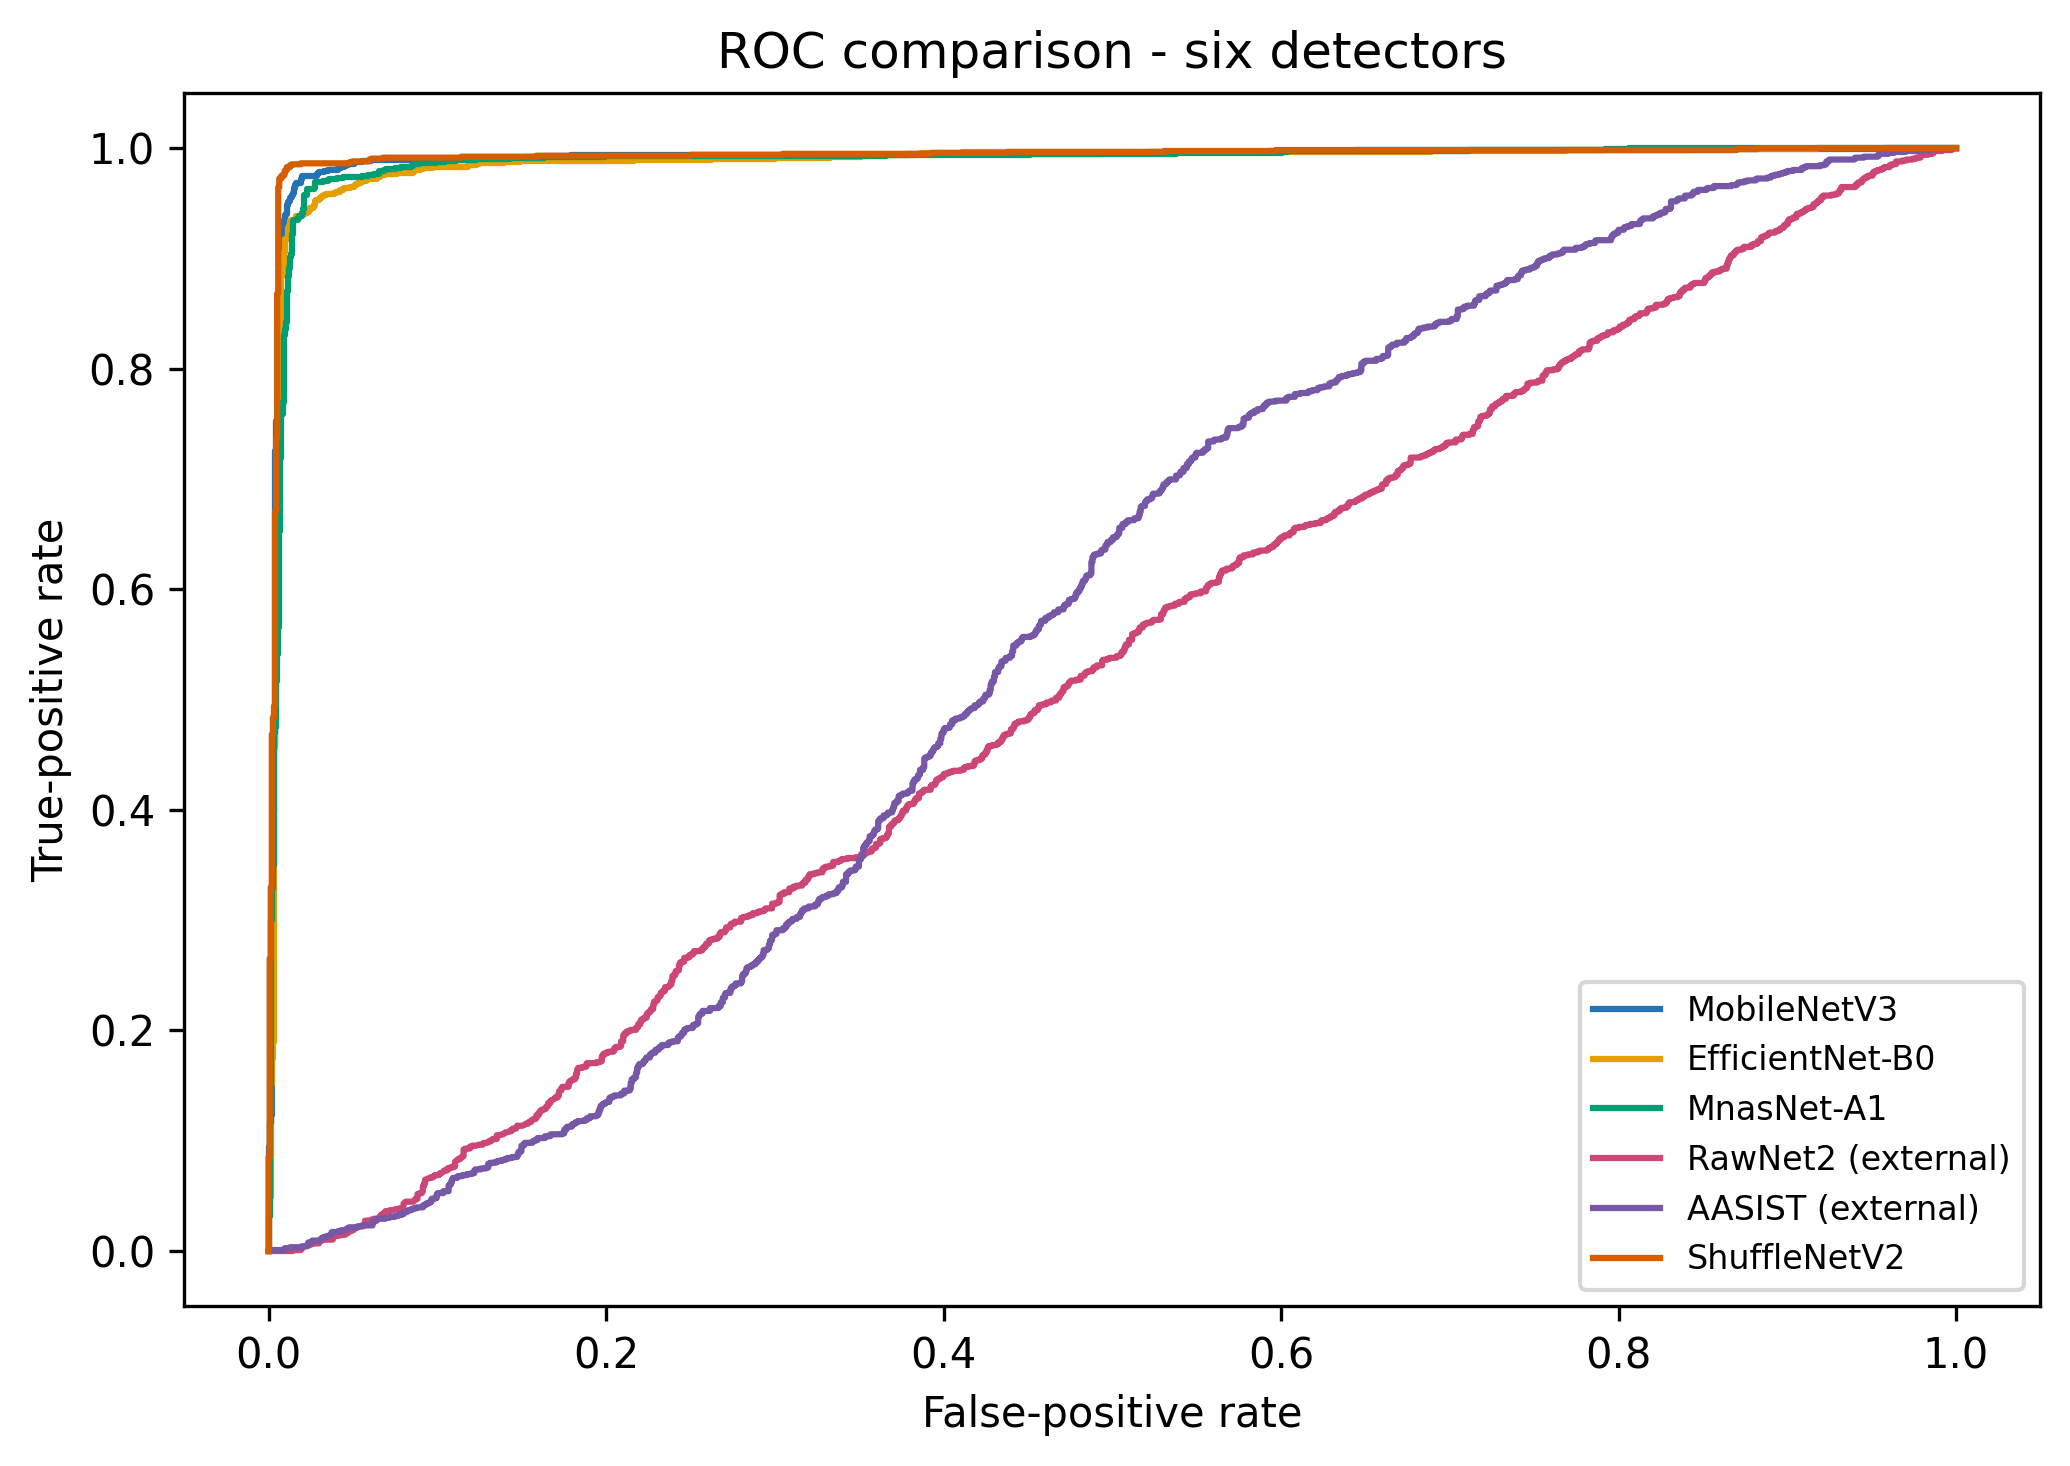
\includegraphics[width=\linewidth]{roc_comparison_6_models.png}\\[-1mm]\small (a) ROC
\end{minipage}\hfill
\begin{minipage}{.49\textwidth}\centering
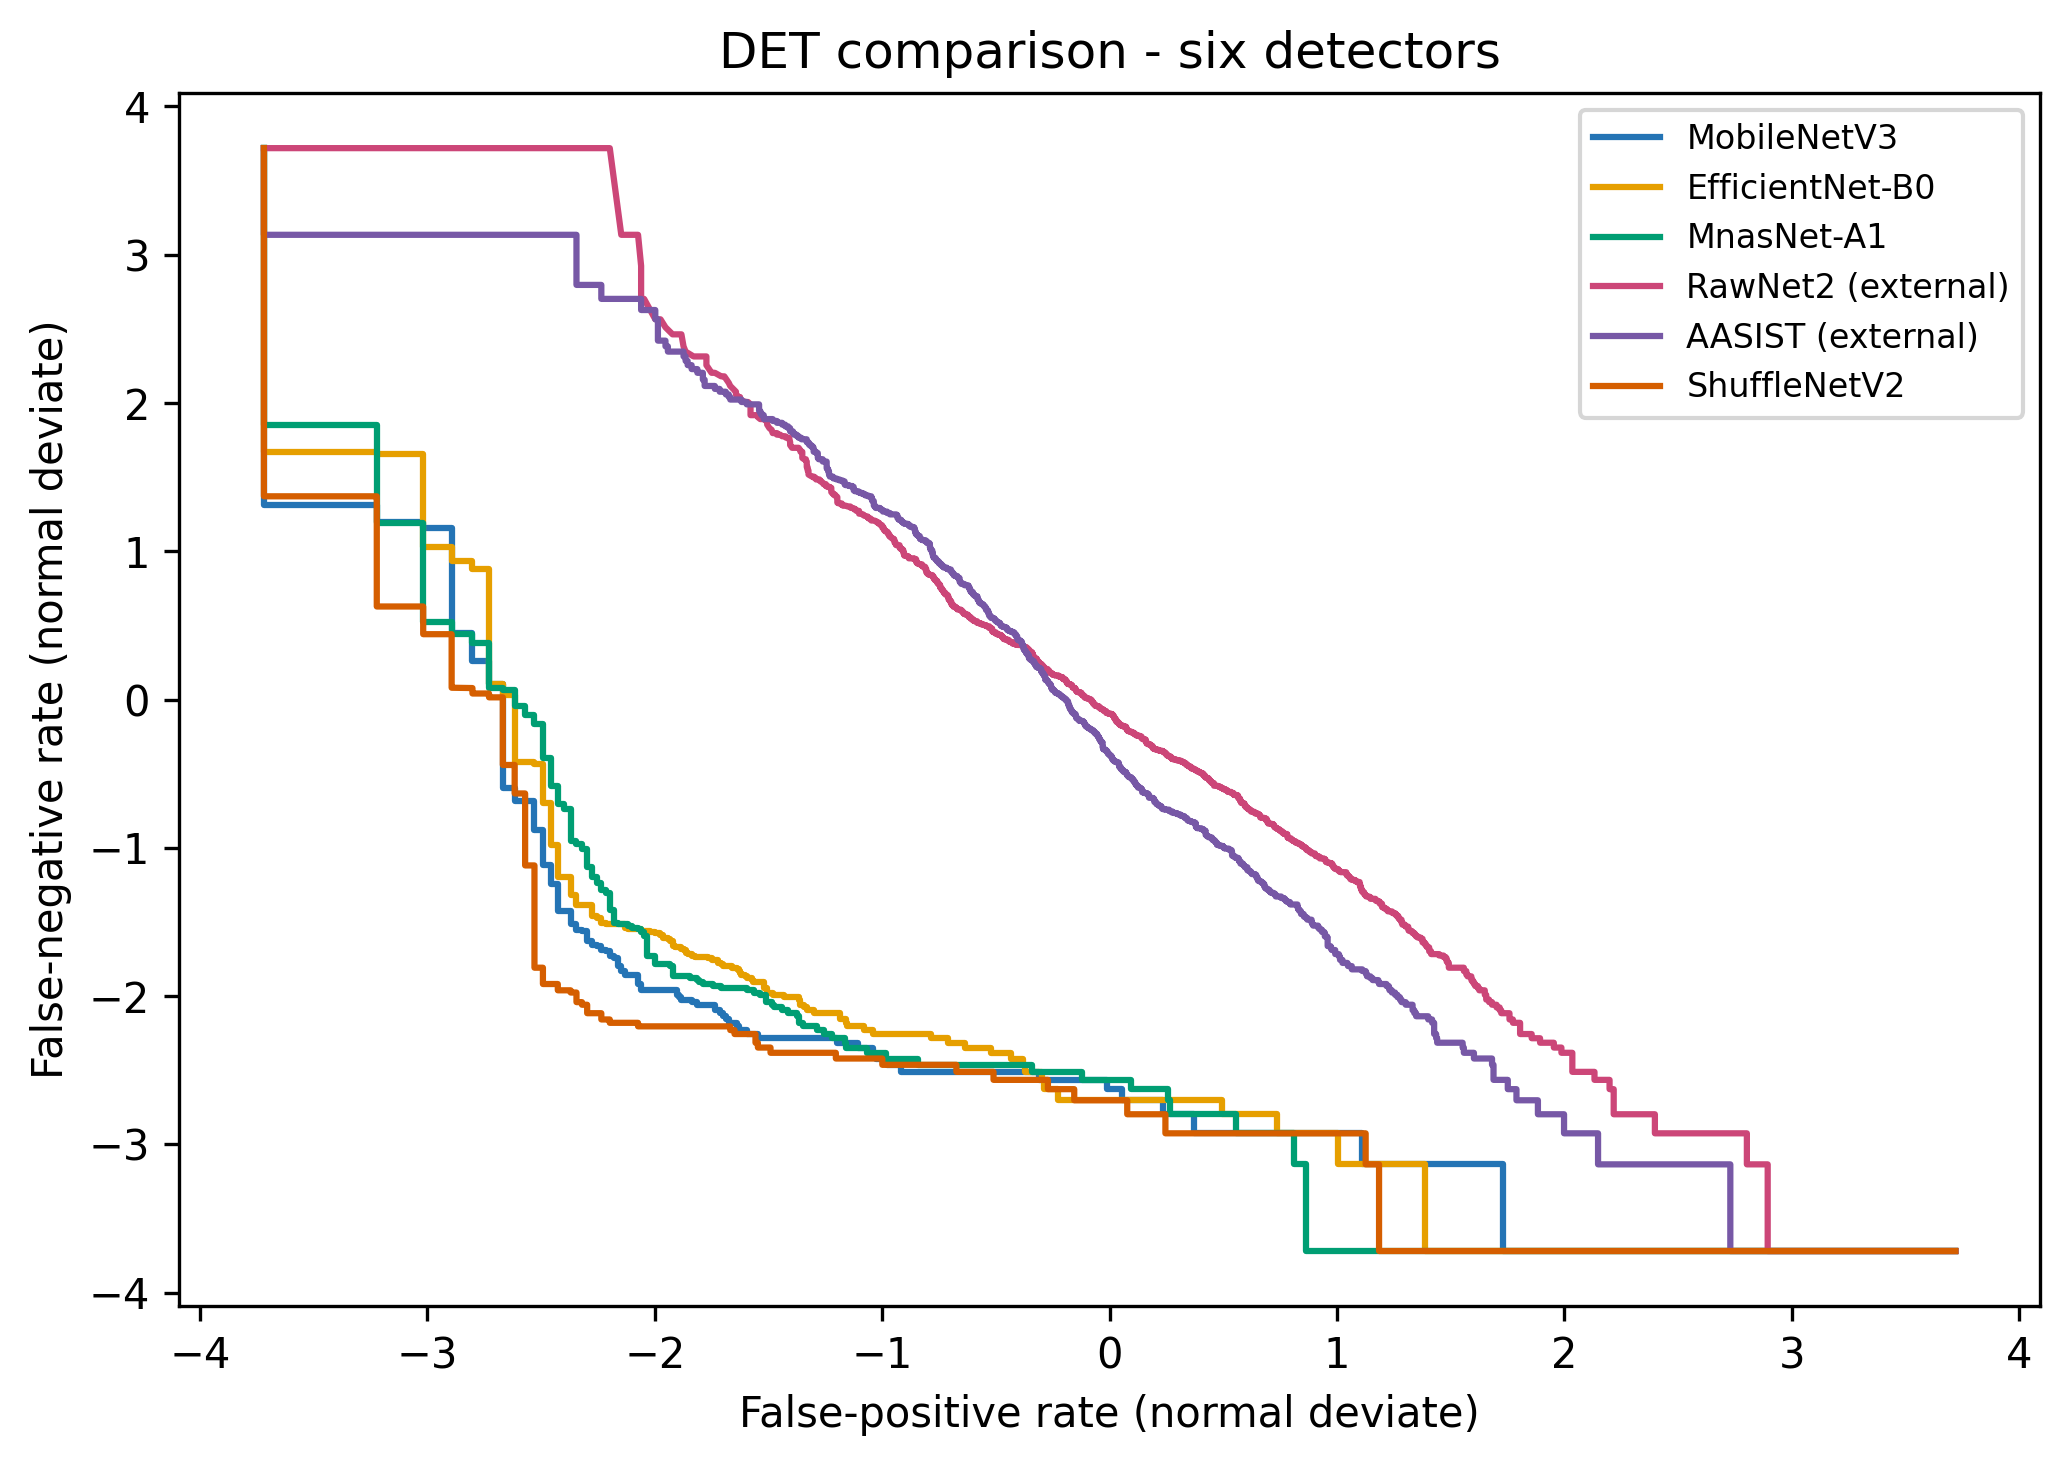
\includegraphics[width=\linewidth]{det_comparison_6_models.png}\\[-1mm]\small (b) DET/EER
\end{minipage}
\caption{Threshold-independent clean discrimination on the full test split.}
\label{fig:clean}
\end{figure}

\subsection{Robustness under Practical Distortions (RQ2)}
Table~\ref{tab:robustness} and Fig.~\ref{fig:robustness} summarize the matched diagnostic. AWGN was the largest weakness for every high-performing lightweight system: mean noise degradation ranged from 0.3555 for ShuffleNet to 0.8053 for EfficientNet and accelerated at 5 and 0 dB. Codec changes were small for the tested settings (0.0000--0.0233 across lightweight models). Under simulated replay, ShuffleNet retained F1 0.9500 ($\Delta$F1 0.0256), compared with degradations 0.0620/0.0641/0.1489 for MobileNet/EfficientNet/MnasNet. Negative reference deltas arise from low baselines and score redistribution; they do not establish superior robustness.

\begin{table}[!t]
\centering\footnotesize
\caption{Diagnostic F1 degradation on the fixed 100-recording subset; lower is better.}
\label{tab:robustness}
\begin{tabularx}{\textwidth}{l r r r r r}
\toprule
Model & Clean F1 & Noise $\Delta$ & Codec $\Delta$ & Replay $\Delta$ & Mean (9) \\
\midrule
MobileNetV3 & .9756 & .6722 & .0095 & .0620 & .3099 \\
ShuffleNetV2 & .9756 & .3555 & .0032 & .0256 & .1623 \\
MnasNet-A1 & .9756 & .6119 & .0233 & .1489 & .2989 \\
EfficientNet-B0 & .9630 & .8053 & .0000 & .0641 & .3650 \\
RawNet2 ext. & .5660 & .5077 & $-.0007$ & $-.0109$ & .2241 \\
AASIST ext. & .5060 & $-.0660$ & $-.0074$ & $-.0682$ & $-.0402$ \\
\bottomrule
\end{tabularx}
\end{table}

\begin{figure}[!t]
\centering
\begin{minipage}{.57\textwidth}\centering
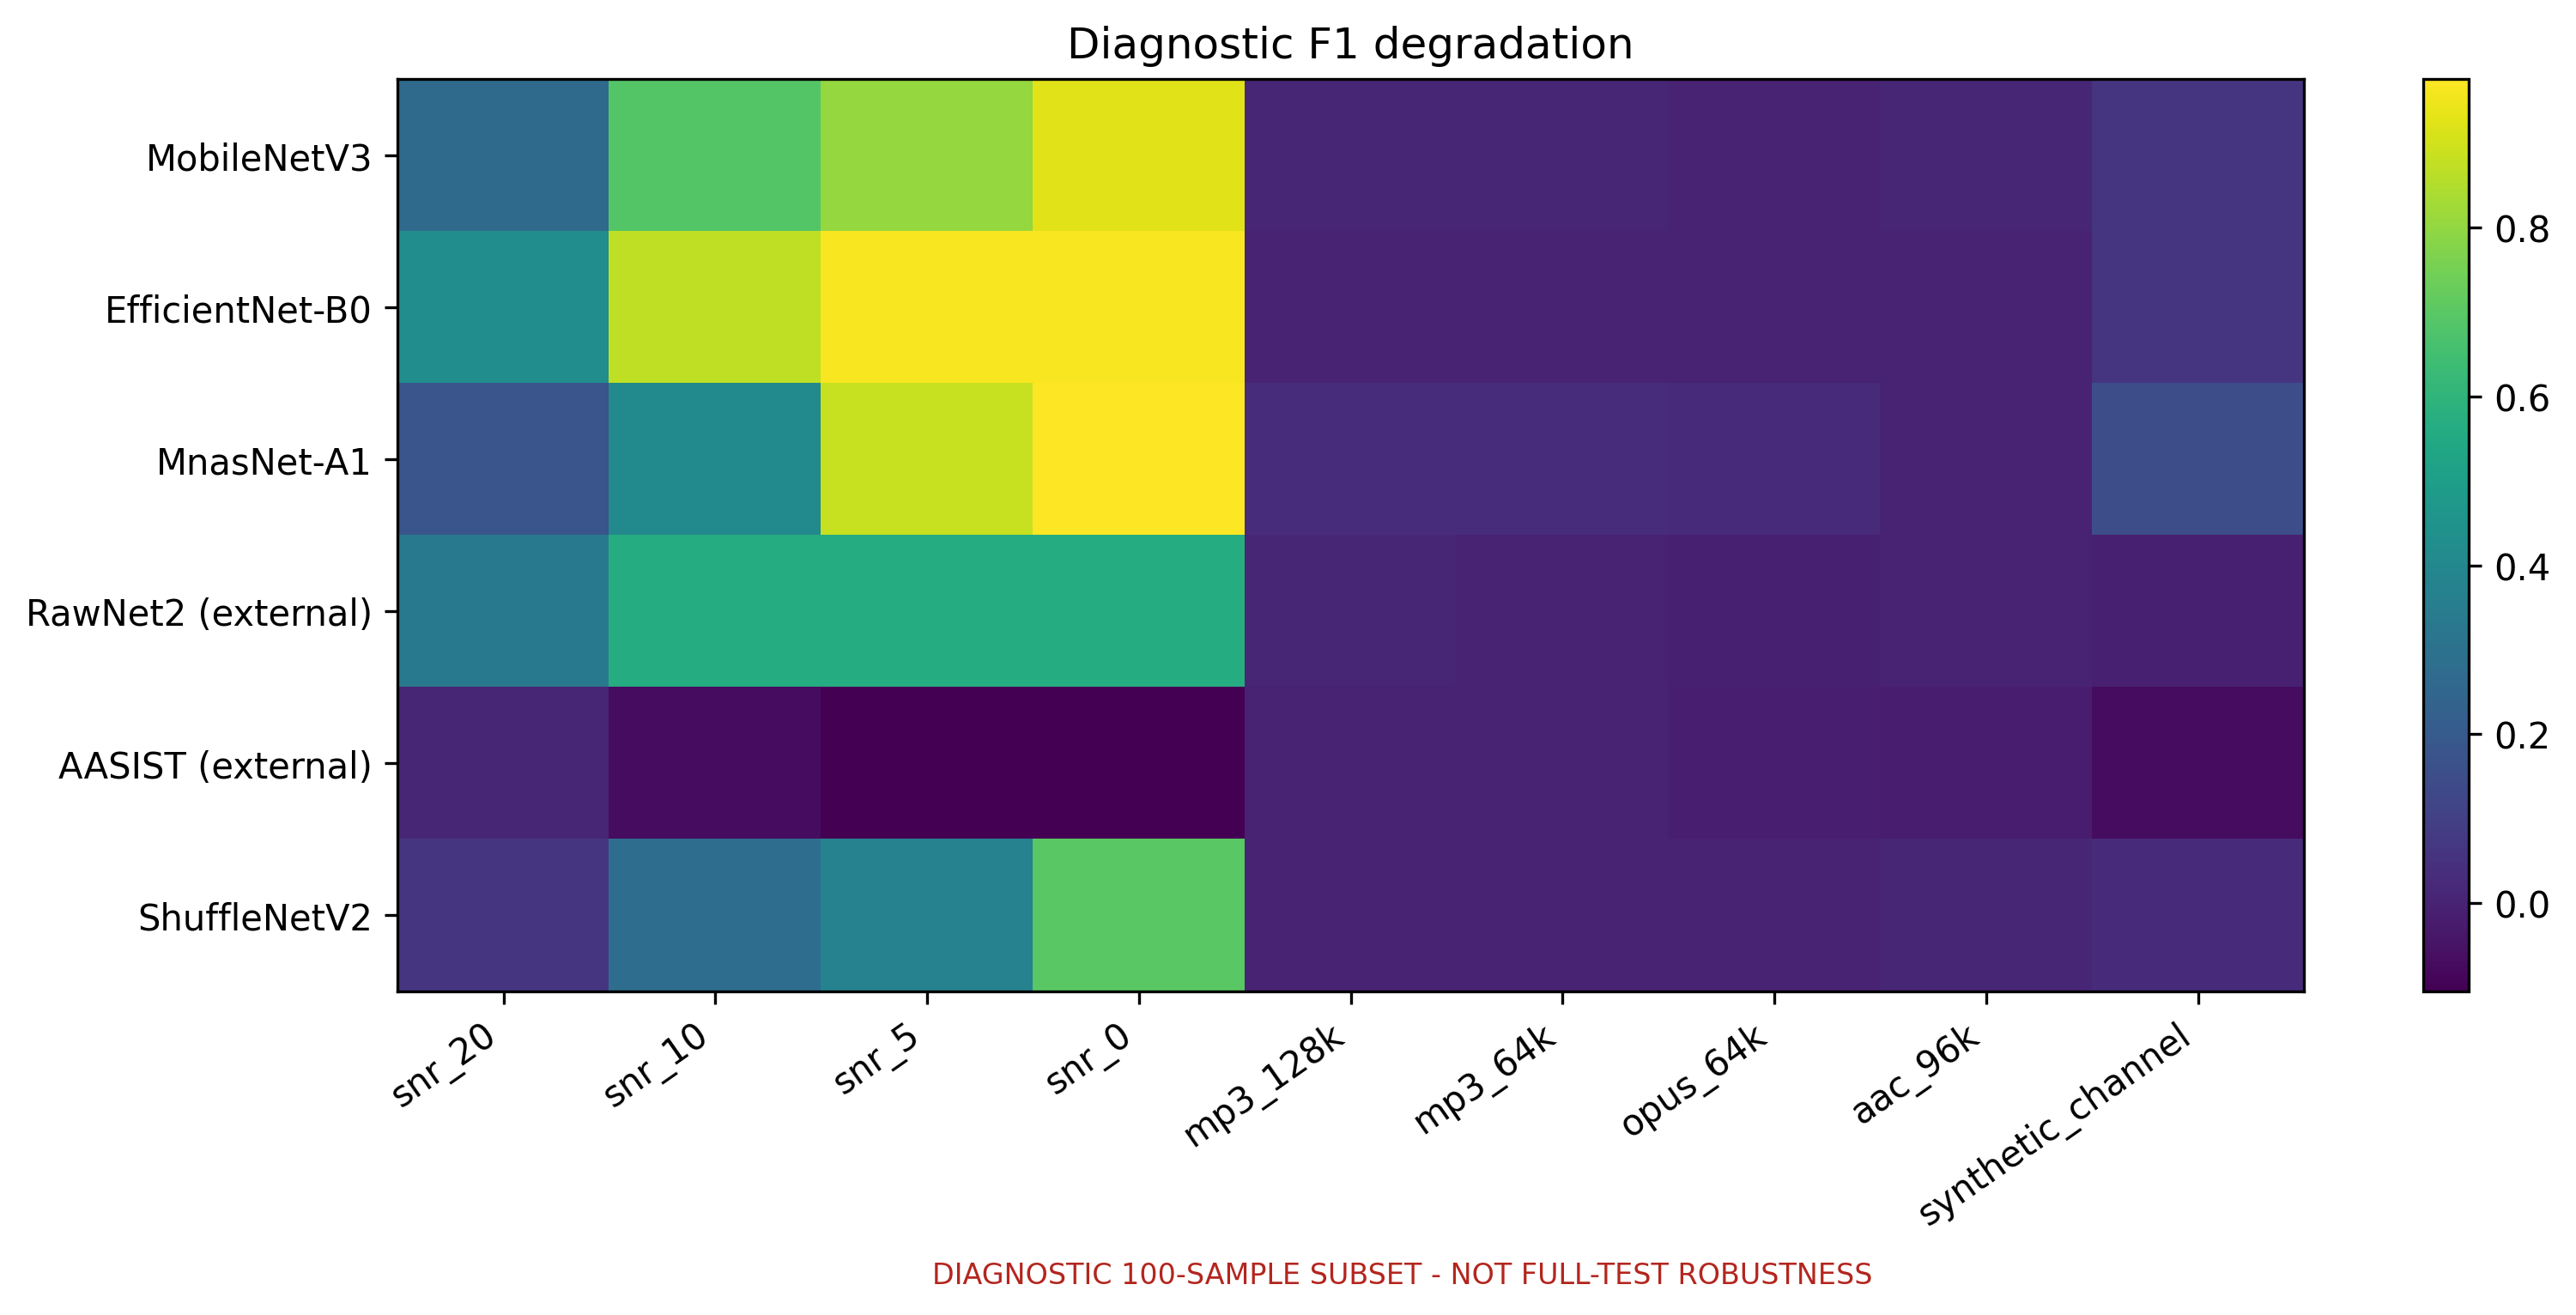
\includegraphics[width=\linewidth]{robustness_heatmap_6_models.png}\\[-1mm]\small (a) Nine-condition degradation
\end{minipage}\hfill
\begin{minipage}{.41\textwidth}\centering
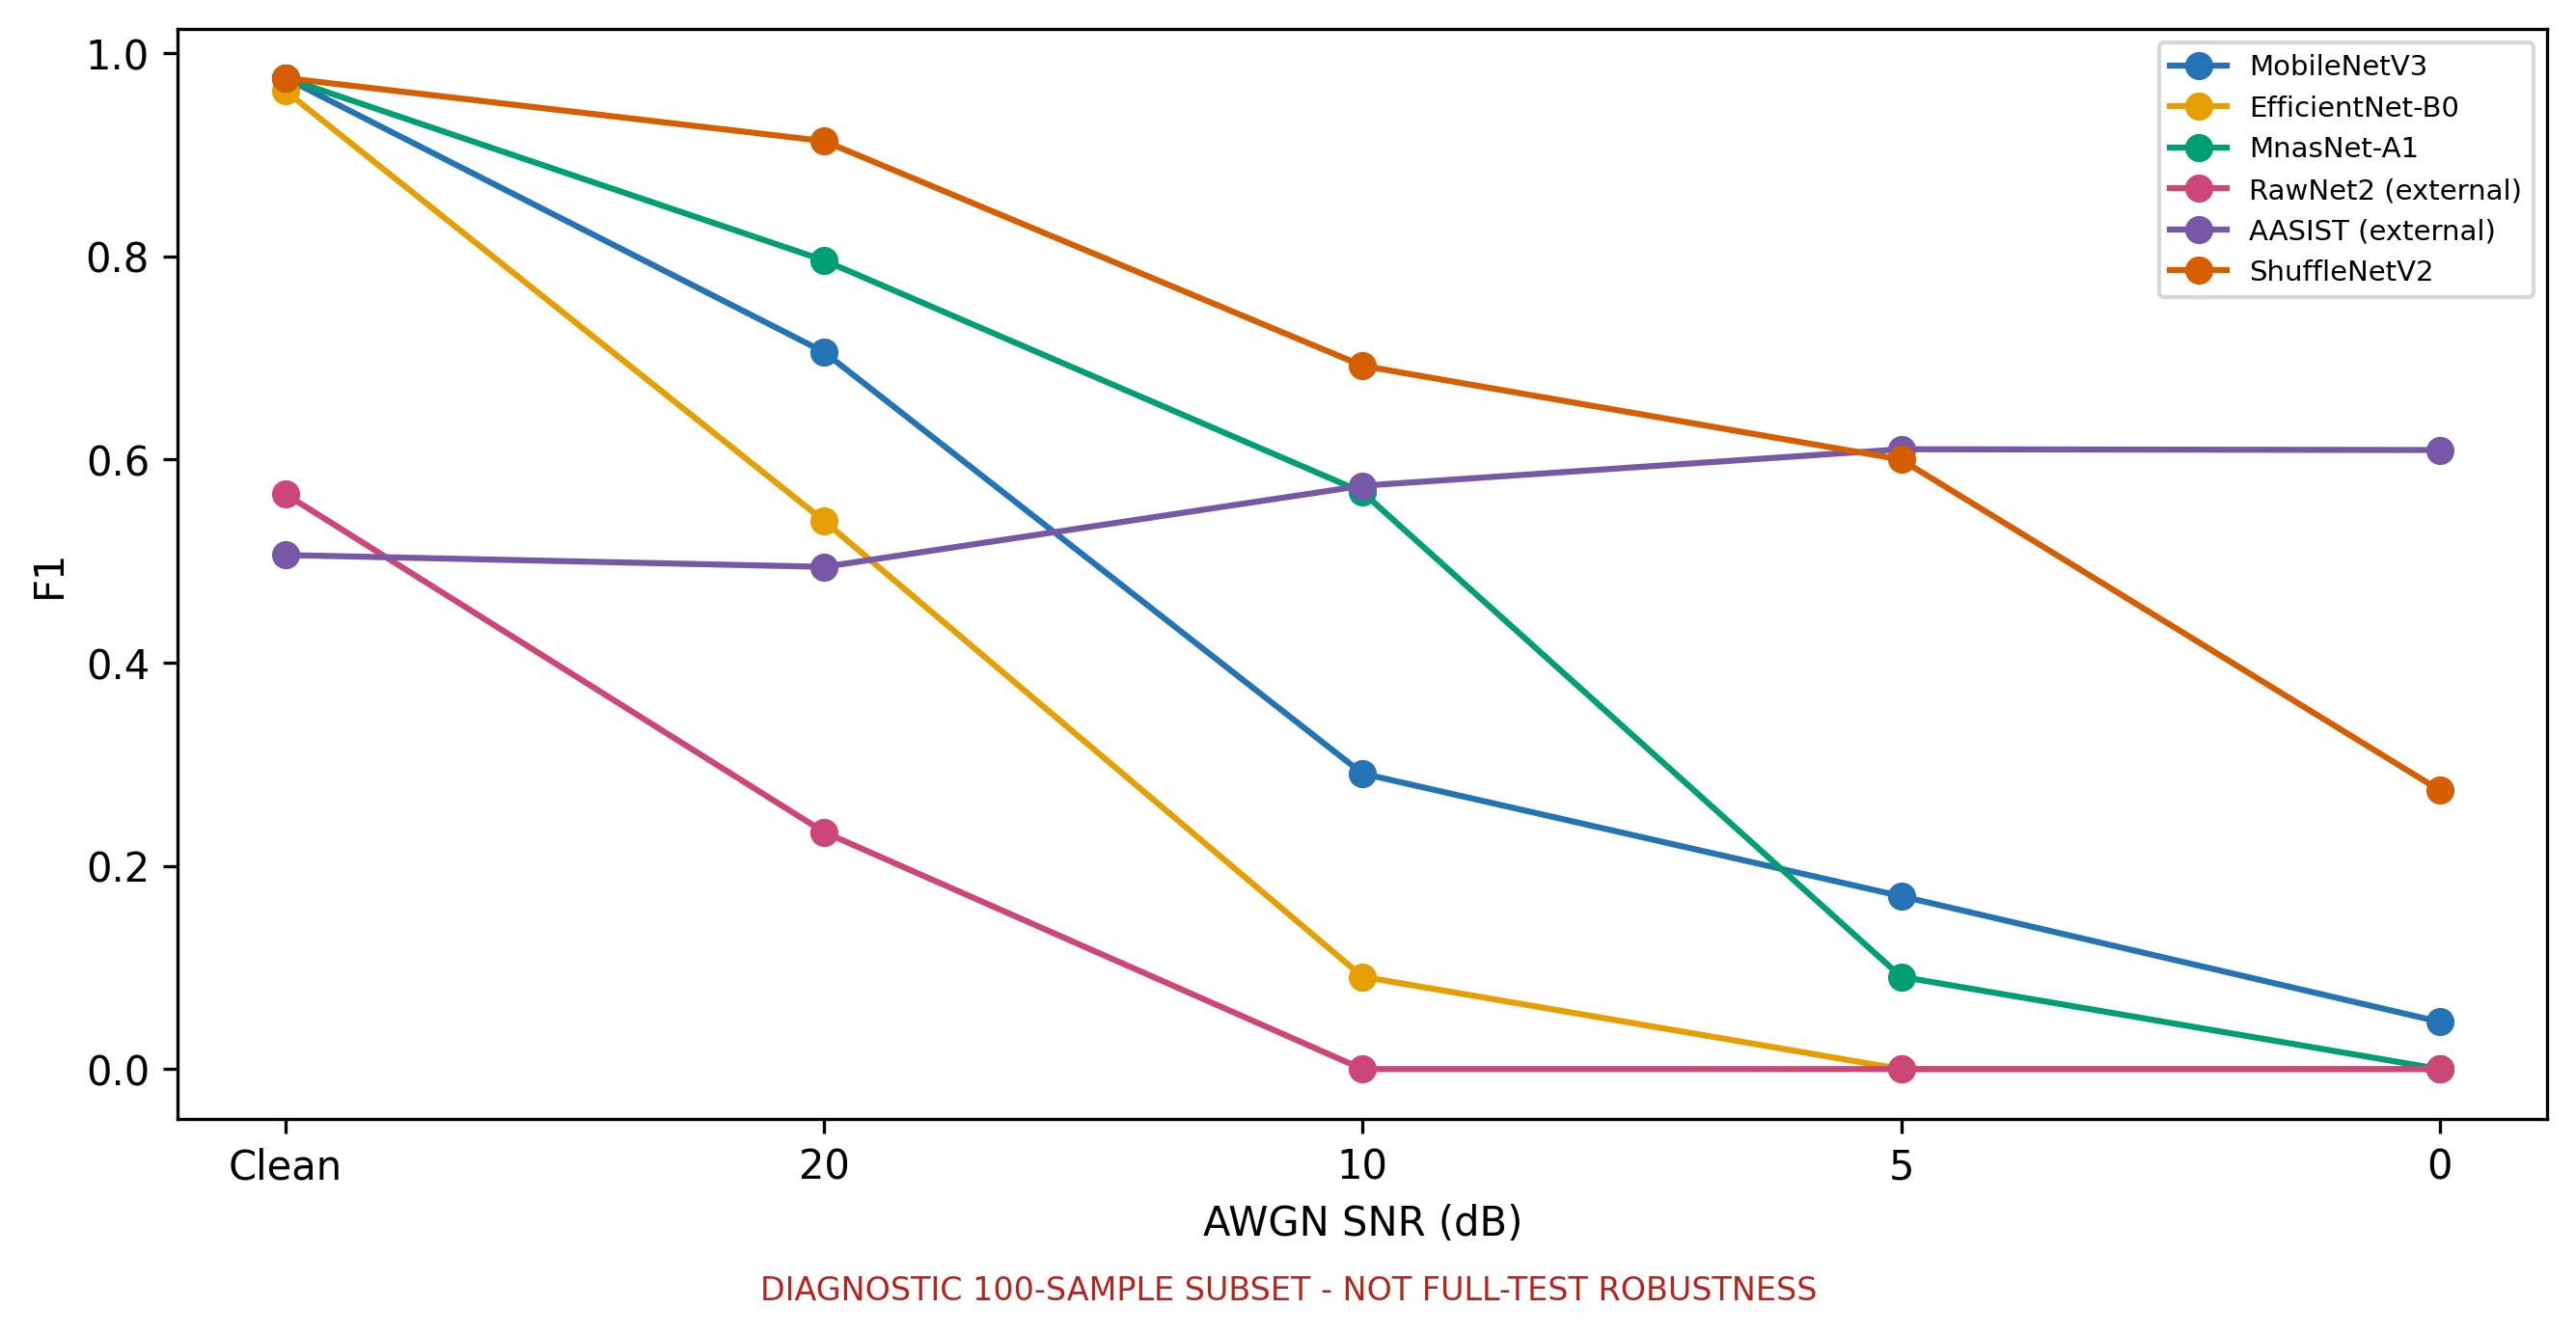
\includegraphics[width=\linewidth]{noise_f1_vs_snr_6_models.png}\\[-1mm]\small (b) AWGN F1 trajectory
\end{minipage}
\caption{Diagnostic robustness; all models reuse identical stressed recordings.}
\label{fig:robustness}
\end{figure}
These outcomes answer RQ2 only for the executed subset and transformations. Codec stability cannot be generalized beyond four round trips, replay is not physical, and no unseen corpus exists.

Condition-level inspection prevents the category means from hiding transitions. Lightweight F1 remained comparatively stable at the mildest noise level but fell sharply toward 5 and 0 dB; the ranking also changed with SNR. The small codec deltas do not imply invariance to transcoding generally, because bitrate, encoder implementation, resampling, packet loss, and tandem compression were not varied. Similarly, the single synthetic impulse response exercises band limitation and delayed energy but not room diversity, playback nonlinearity, microphone response, or distance.

Across all nine conditions, the lightweight mean degradations were 0.1623 (ShuffleNet), 0.2989 (MnasNet), 0.3099 (MobileNet), and 0.3650 (EfficientNet). AASIST's value of $-0.0402$ is mathematically lower but accompanies clean-subset F1 0.5060; it illustrates why degradation must be paired with absolute performance. RawNet2 likewise improved slightly under the codec/replay transforms but retained subset-clean F1 0.5660. The diagnostic design supports failure-mode discovery and controlled cross-model comparison, not population-level robustness confidence intervals.

\subsection{Computational Efficiency}
Under the common single-thread CPU protocol (Table~\ref{tab:efficiency}), MobileNet had the lowest latency and RTF; ShuffleNet was second among TensorFlow detectors. AASIST combined the smallest artifact with the largest latency, whereas RawNet2 combined the largest parameter count with moderate latency. Parameters and serialized size therefore did not predict runtime. RSS is whole-process memory, not model-only tensor allocation.

Preprocessing averaged 13.43, 15.57, 13.60, and 13.59 ms for MobileNet, ShuffleNet, MnasNet, and EfficientNet; their corresponding model-only means were 30.07, 48.05, 95.25, and 168.36 ms. Waveform preparation was only 0.63/0.47 ms for RawNet2/AASIST, while model-only time was 95.10/359.61 ms. The contrast demonstrates why timing only preprocessing, parameter count, or nominal architecture complexity would misrepresent deployment cost.

\begin{table}[!t]
\centering\scriptsize
\caption{Measured float32 batch-one desktop-CPU efficiency (10 warm-ups, 50 runs).}
\label{tab:efficiency}
\begin{tabularx}{\textwidth}{l r r r r r r r}
\toprule
Model & Params & MiB & RSS & E2E ms & P95 ms & clips/s & RTF \\
\midrule
MobileNetV3 & 1.31M & 5.64 & 554.6 & 43.81 & 52.12 & 22.83 & .0146 \\
ShuffleNetV2 & 1.87M & 7.74 & 501.8 & 62.52 & 75.37 & 15.99 & .0208 \\
MnasNet-A1 & 3.37M & 13.43 & 566.0 & 117.00 & 138.96 & 8.55 & .0390 \\
EfficientNet-B0 & 4.78M & 18.96 & 651.2 & 175.85 & 196.11 & 5.69 & .0586 \\
RawNet2 ext. & 17.62M & 67.65 & 249.5 & 96.54 & 102.62 & 10.36 & .0239 \\
AASIST ext. & .30M & 1.61 & 442.5 & 362.91 & 398.45 & 2.76 & .0899 \\
\bottomrule
\end{tabularx}
\end{table}

\begin{figure}[!t]
\centering
\begin{minipage}{.49\textwidth}\centering
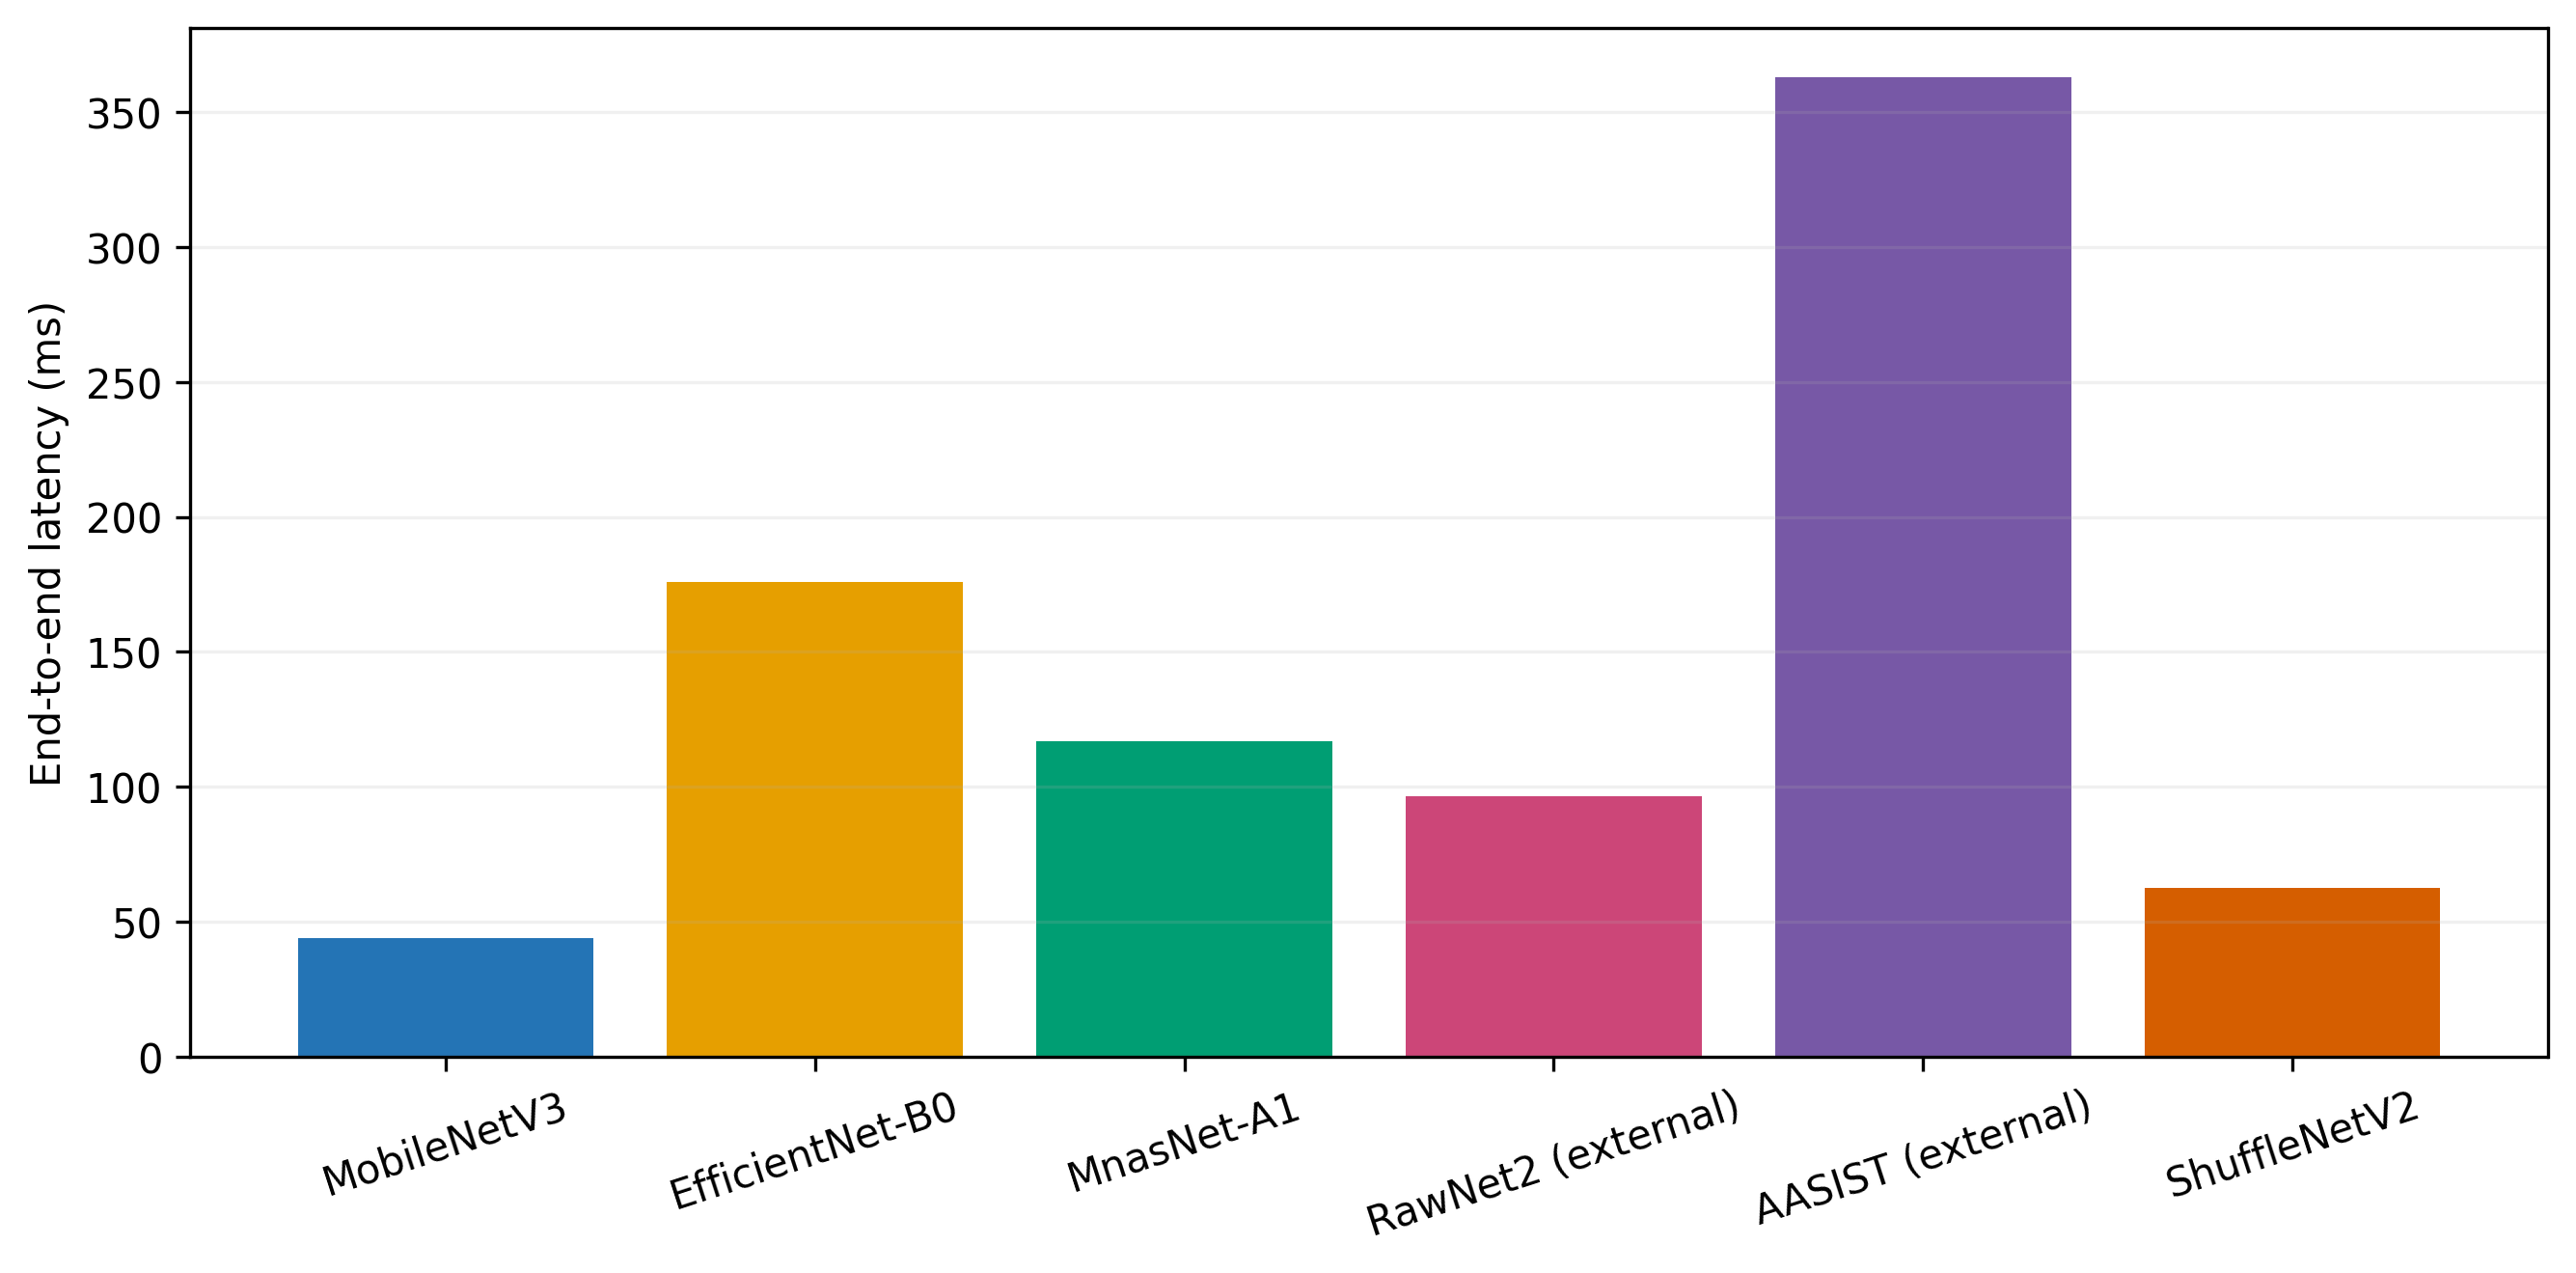
\includegraphics[width=\linewidth]{end_to_end_latency_bar_6_models.png}\\[-1mm]\small (a) End-to-end latency
\end{minipage}\hfill
\begin{minipage}{.49\textwidth}\centering
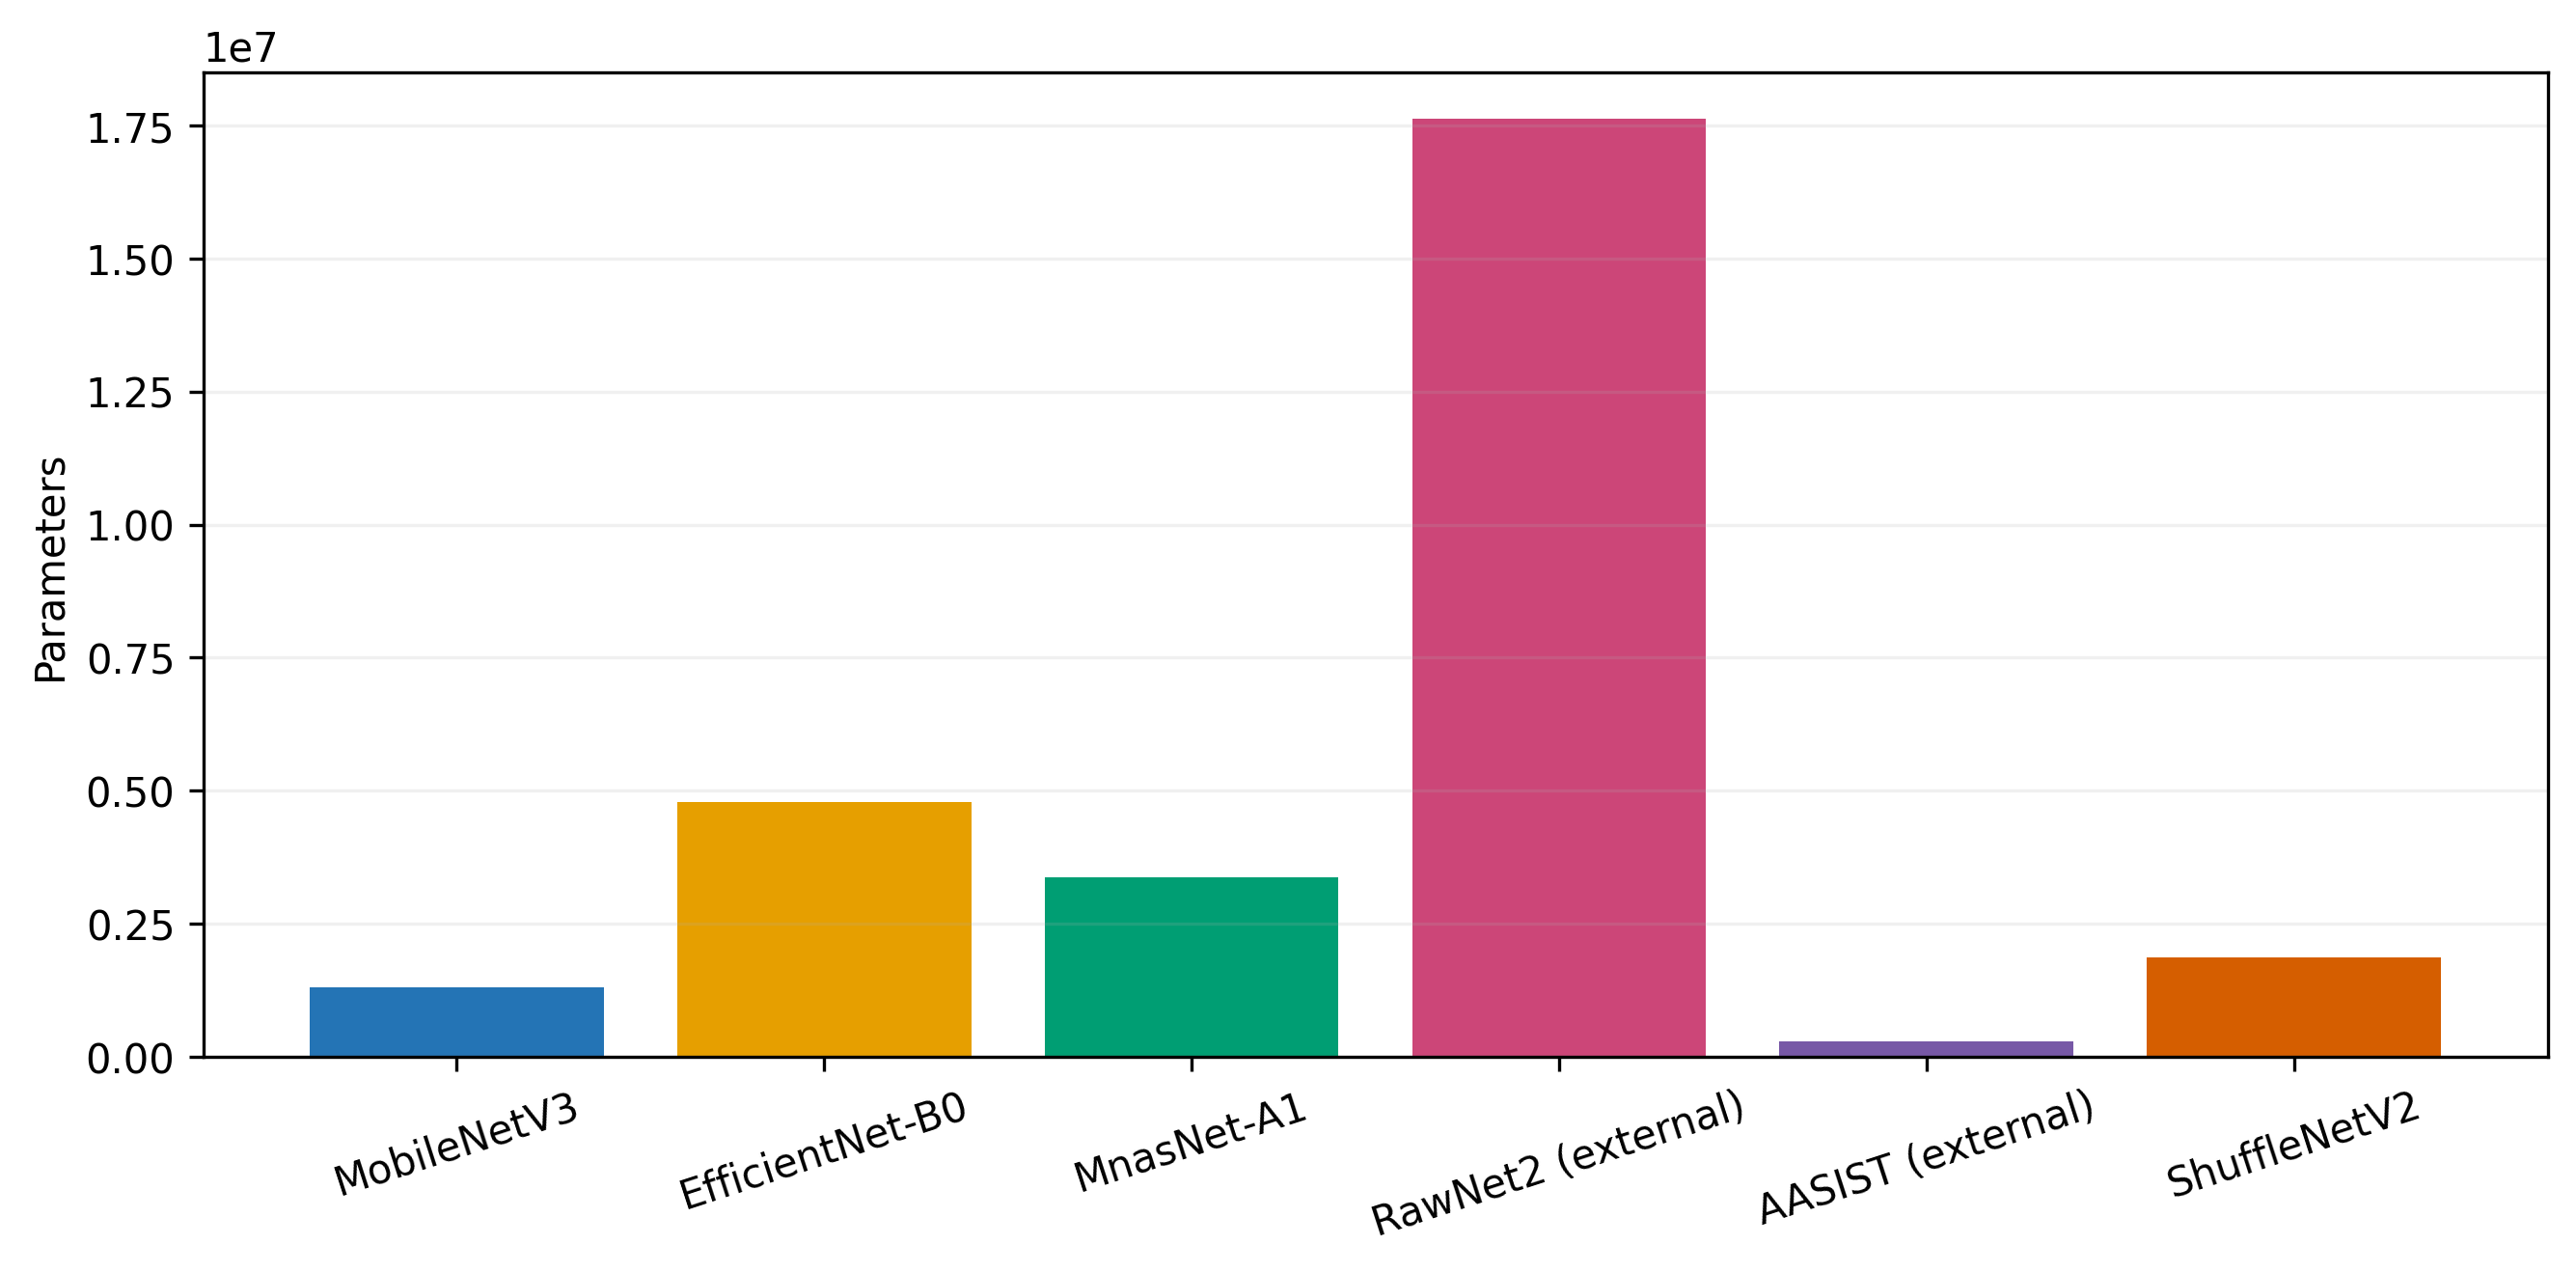
\includegraphics[width=\linewidth]{parameters_bar_6_models.png}\\[-1mm]\small (b) Parameter count
\end{minipage}
\caption{Runtime and complexity are related but not interchangeable.}
\label{fig:efficiency}
\end{figure}
All measured RTFs are below 0.1, supporting faster-than-duration offline inference on this CPU, not continuous streaming or edge deployment.

Whole-process RSS ranged from 249.5 MiB for RawNet2 to 651.2 MiB for EfficientNet. MobileNet and ShuffleNet consumed 554.6 and 501.8 MiB, respectively, despite serialized artifacts of only 5.64 and 7.74 MiB; framework and allocator state dominate that difference. P95 overhead relative to the mean was 8.31 ms for MobileNet, 12.85 ms for ShuffleNet, 21.96 ms for MnasNet, 20.26 ms for EfficientNet, 6.08 ms for RawNet2, and 35.54 ms for AASIST. These distributions reinforce the need to report tail as well as mean latency.

\subsection{Pareto Trade-Offs (RQ3)}
The non-dominated diagnostic set is MobileNet, ShuffleNet, and AASIST (Table~\ref{tab:pareto}, Fig.~\ref{fig:pareto}). MobileNet supplies the lowest RTF; ShuffleNet combines the same subset EER with lower degradation at a modest latency cost. AASIST remains non-dominated only because negative degradation from a weak clean baseline occupies an extreme coordinate. Frontier membership is not a scalar ranking. ShuffleNet dominates MnasNet and RawNet2; MobileNet dominates EfficientNet under these objectives.

The first four lightweight models share diagnostic subset EER 0.0476, so their frontier relations are driven by robustness degradation and RTF. ShuffleNet improves mean degradation by 0.1476 over MobileNet but increases RTF by 0.0062; neither dominates the other. MnasNet has slightly lower degradation than MobileNet but loses on RTF and does not improve EER relative to ShuffleNet, while EfficientNet is worse than MobileNet on both degradation and RTF. These statements refer to the fixed objective vector and do not imply a preferred deployment without application constraints.

\begin{table}[!t]
\centering\footnotesize
\caption{Exploratory three-objective Pareto result on the diagnostic scope.}
\label{tab:pareto}
\begin{tabularx}{\textwidth}{l r r r c}
\toprule
Model & Subset EER & Mean $\Delta$F1 & RTF & Frontier \\
\midrule
MobileNetV3 & .0476 & .3099 & .0146 & Yes \\
ShuffleNetV2 & .0476 & .1623 & .0208 & Yes \\
MnasNet-A1 & .0476 & .2989 & .0390 & No \\
EfficientNet-B0 & .0476 & .3650 & .0586 & No \\
RawNet2 ext. & .4138 & .2241 & .0239 & No \\
AASIST ext. & .3810 & $-.0402$ & .0899 & Yes \\
\bottomrule
\end{tabularx}
\end{table}

\begin{figure}[!t]
\centering
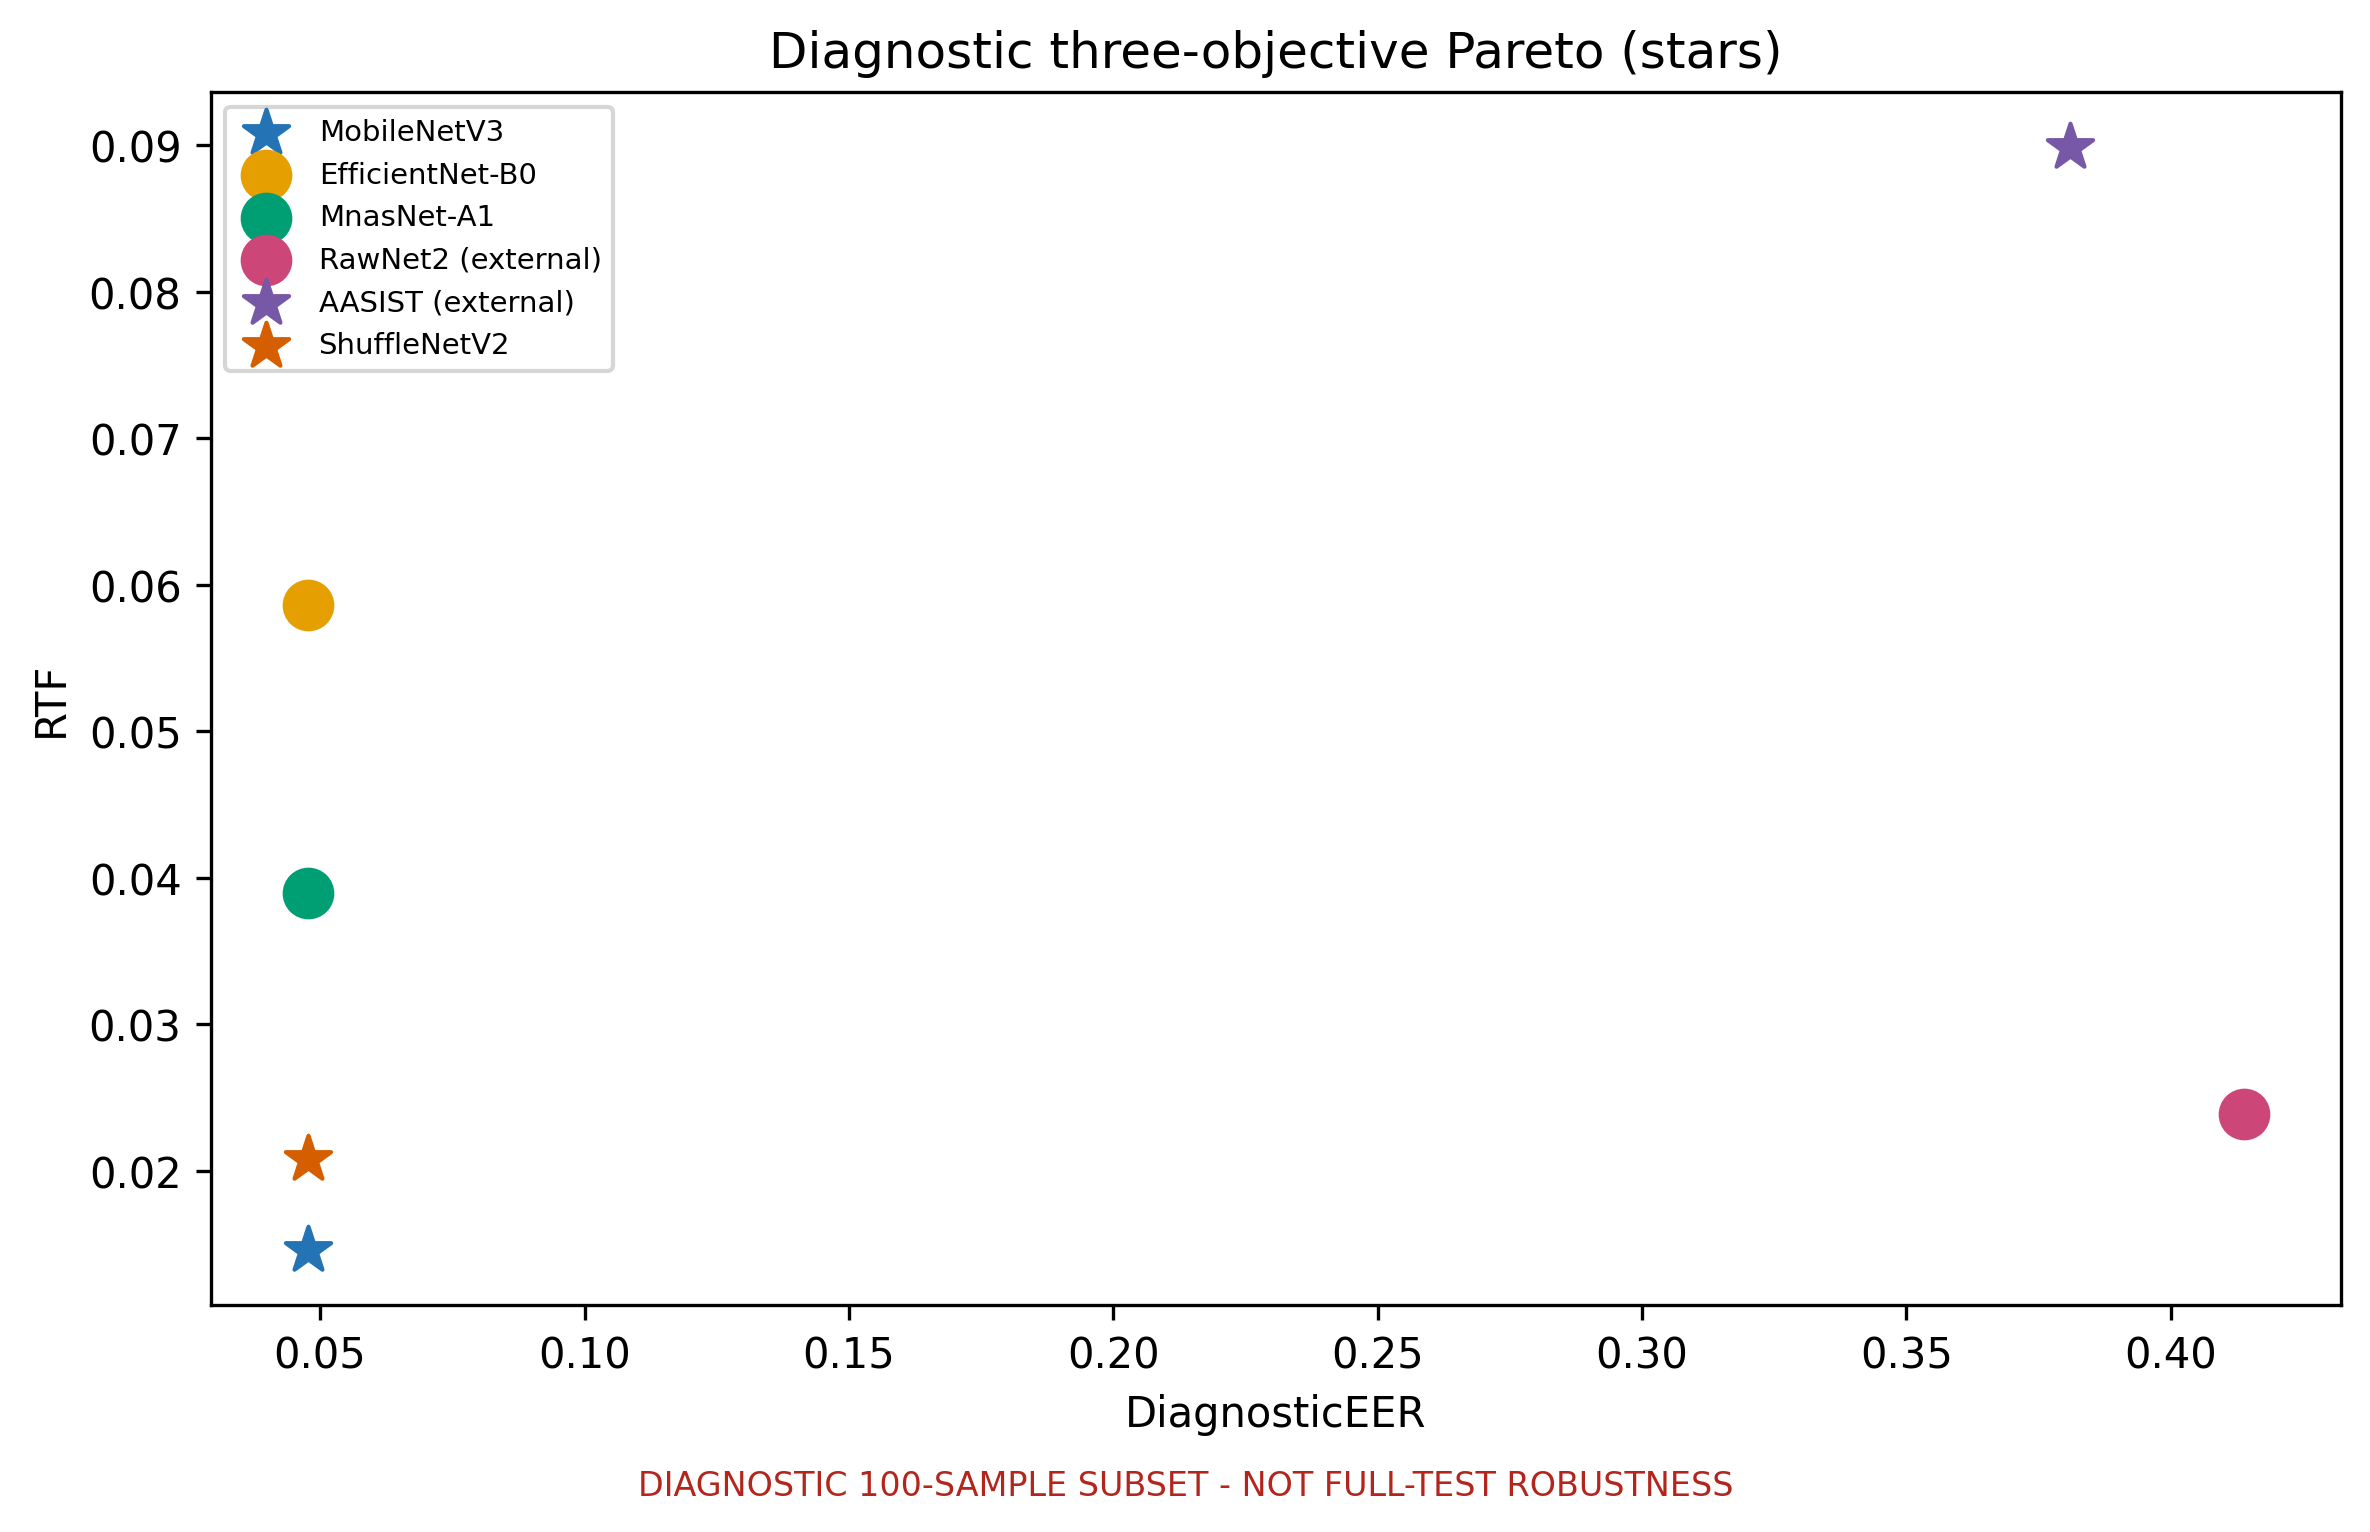
\includegraphics[width=.72\textwidth]{pareto_eer_rtf_6_models.png}
\caption{EER--RTF projection; stars mark the three-objective diagnostic frontier.}
\label{fig:pareto}
\end{figure}
Because robustness is diagnostic, RQ3 is exploratory. A full-test stress run, new hardware, or another threshold policy can change the frontier.

\subsection{Error, Agreement, and Statistical Evidence}
All six detectors were correct on 911 clean samples and wrong on 10. The four lightweight models were unanimously correct while both references were wrong on 785 samples; the reverse occurred on three. ShuffleNet agreed with MobileNet/EfficientNet/MnasNet on 0.979/0.970/0.977 of decisions, but with RawNet2/AASIST on 0.494/0.559; agreement does not imply correctness.

Full-test 95\% bootstrap intervals for ShuffleNet were [0.9768, 0.9875] for F1, [0.9894, 0.9960] for AUC, and [0.0103, 0.0207] for EER. In the 15-pair McNemar family, ShuffleNet differed from MobileNet after Holm correction ($p_{adj}=0.0096$) and more strongly from EfficientNet and MnasNet. MobileNet--MnasNet ($p_{adj}=0.1060$) and EfficientNet--MnasNet ($p_{adj}=0.1180$) were not significant at 0.05; every lightweight--reference comparison was significant. Complete six-model intervals, paired F1 differences, adjusted $p$-values, agreement, and error matrices remain in supplementary artifacts.

For completeness, the corresponding F1 intervals were [0.9654,0.9788] for MobileNet, [0.9573,0.9717] for MnasNet, [0.9477,0.9651] for EfficientNet, [0.5150,0.5489] for RawNet2, and [0.4928,0.5349] for AASIST. AUC intervals were [0.9871,0.9947], [0.9842,0.9923], [0.9833,0.9917], [0.4944,0.5395], and [0.5377,0.5815], respectively. These intervals quantify finite-test sampling conditional on the existing checkpoints; they cannot measure training-seed variation.

EER intervals were [0.0178,0.0311] for MobileNet, [0.0250,0.0379] for MnasNet, [0.0311,0.0482] for EfficientNet, [0.4616,0.5016] for RawNet2, and [0.4279,0.4660] for AASIST. Pairwise F1-difference intervals for ShuffleNet minus MobileNet/EfficientNet/MnasNet were [0.0036,0.0166], [0.0182,0.0339], and [0.0116,0.0247]. Their corresponding discordant correctness counts (ShuffleNet wrong/right) were 17/40, 12/71, and 10/52. The direction and paired evidence agree with the clean table, while the non-significant MobileNet--MnasNet and EfficientNet--MnasNet comparisons discourage over-ordering the middle lightweight systems.

The overlap analysis adds a complementary systems view. Unanimous correctness on 911 recordings indicates a core region handled by every artifact despite provenance differences, whereas 10 unanimous failures identify candidates for waveform, metadata, and generator-level inspection. The 785 cases where every lightweight detector was correct and both references were wrong dominate the between-stratum disagreement; only three samples show the reverse pattern. This asymmetry is compatible with dataset adaptation, but without source/generator annotations it cannot establish which acoustic factors drive the failures. Future error studies should therefore enrich the manifest rather than treating disagreement alone as a causal explanation.

From a deployment perspective, MobileNet and ShuffleNet define the most practically attractive measured region: both combine high clean discrimination with sub-0.021 RTF, while ShuffleNet provides better clean and diagnostic robustness outcomes at a modest latency cost. EfficientNet's larger artifact and higher latency do not improve clean quality in its available warm-up state. MnasNet remains competitive in detection but is dominated in the current diagnostic objectives. The reference systems remain scientifically useful as heterogeneous stress tests for the adapter and score contract even though their absolute clean results are weak. These conclusions should be revisited after validation calibration of the references, multi-seed lightweight training, and target-hardware measurement.

\begin{figure}[!t]
\centering
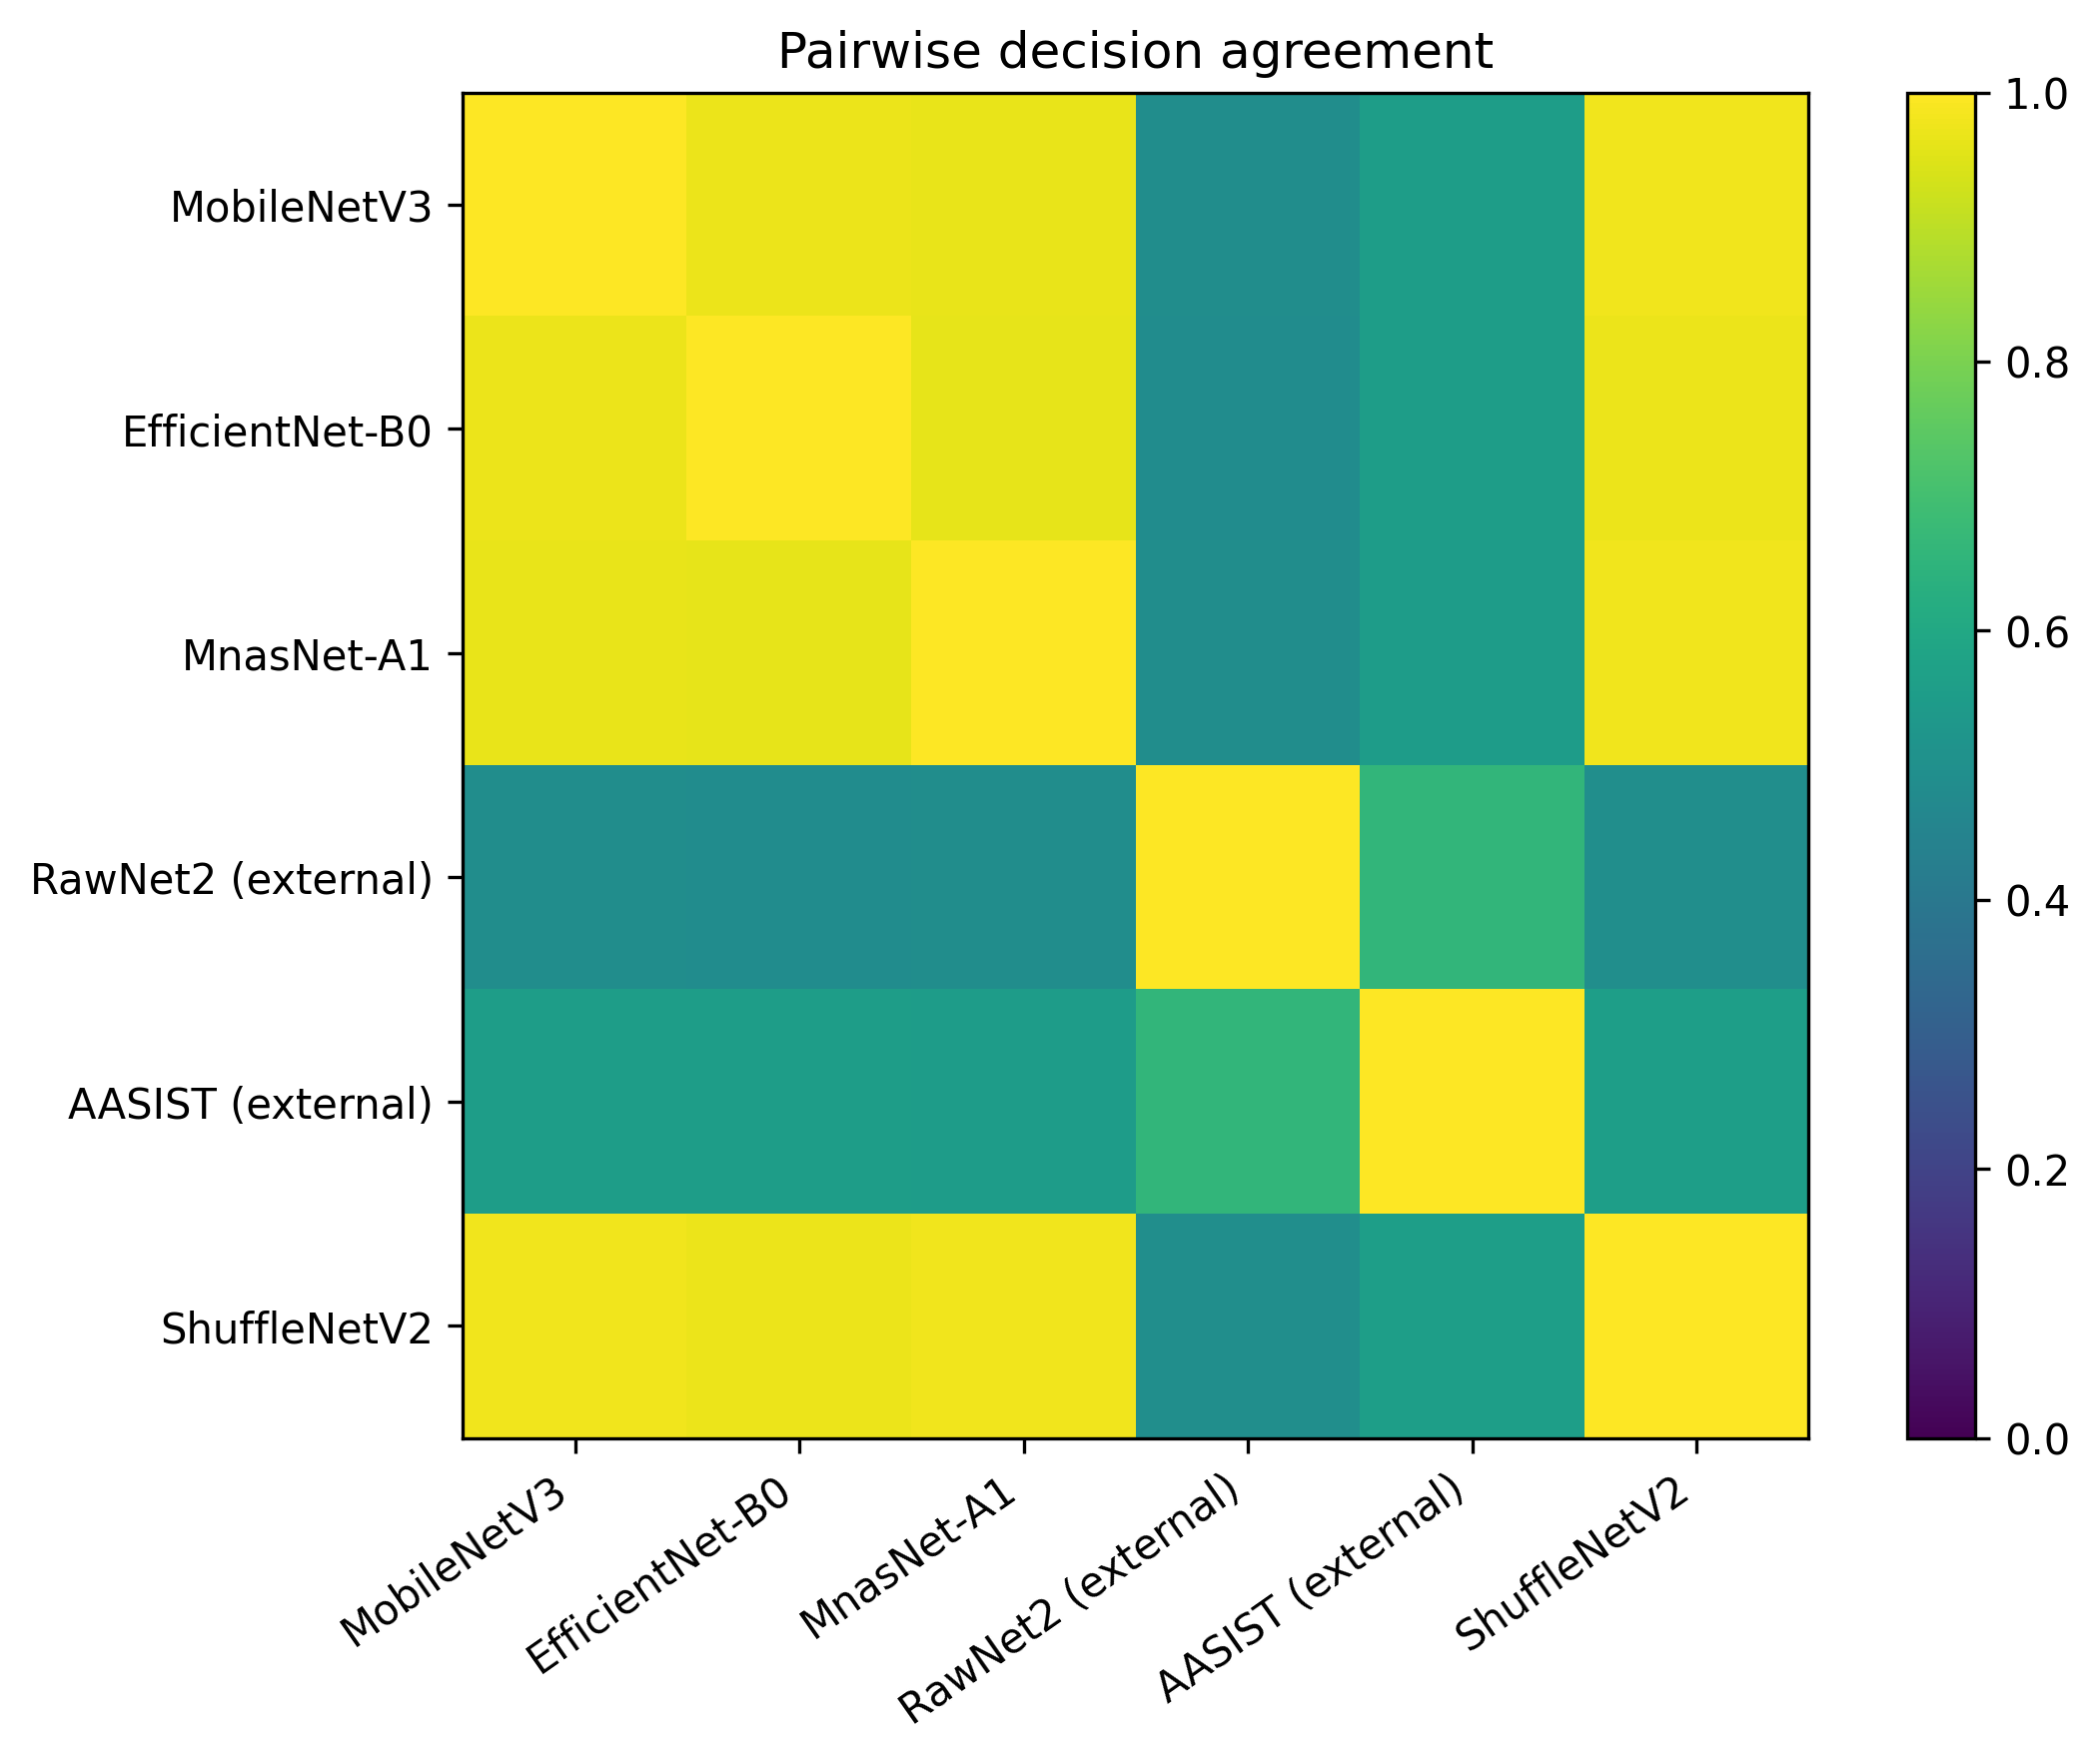
\includegraphics[width=.68\textwidth]{agreement_heatmap_6_models.png}
\caption{Pairwise agreement on identical full-test sample IDs; agreement is not accuracy.}
\label{fig:agreement}
\end{figure}

\subsection{Direct Answers to the Research Questions}
\textbf{RQ1:} the four locally trained lightweight artifacts outperform the two external references under this clean contract, with ShuffleNet strongest in detection and MobileNet fastest. \textbf{RQ2:} codec and simulated-replay changes were modest relative to low-SNR white noise, but evidence is limited to 100 matched samples. \textbf{RQ3:} MobileNet, ShuffleNet, and AASIST are non-dominated in the diagnostic space; AASIST's membership reflects a negative degradation coordinate rather than strong absolute detection. These findings characterize artifacts under LAVA, not universally superior architectures.

\section{Limitations}
The study mixes ImageNet transfer (MobileNet/EfficientNet), scratch optimization (ShuffleNet/MnasNet), and external RawNet2/AASIST checkpoints, so evaluation consistency is not identical training. Missing speaker/source/generator identifiers permit only checksum-group-disjoint claims. Robustness uses 100 samples; replay is simulated; no unseen corpus, physical replay, codec-version seal, or probability calibration exists. Runtime was measured on one desktop CPU rather than an edge target, and single checkpoints plus test-set bootstrap do not replace multi-seed training. Future work should first execute full-test stresses and a metadata-rich external corpus, then measure physical replay and target hardware before quantization or streaming studies.

\section{Conclusion}
LAVA provides an evidence-traceable interface for six architecturally heterogeneous voice anti-spoofing artifacts. On 2,737 clean test recordings, ShuffleNetV2-LSTM delivered the best F1/AUC/EER, while MobileNetV3Small-LSTM minimized latency and RTF. The diagnostic stresses identify low-SNR noise as the principal weakness, and multi-objective analysis retains MobileNet, ShuffleNet, and AASIST for different trade-offs. These results support reproducible deployment-oriented comparison and faster-than-duration offline inference, not unseen-domain, physical-replay, streaming, or edge-device validation.

\section{Acknowledgements}
This research is supported by the University of Economics Ho Chi Minh City, Vietnam (UEH).

\bibliographystyle{IEEEtran}
\bibliography{references}
\end{document}
